\documentclass[11pt]{article}

\usepackage[review]{acl}

\usepackage{times}
\usepackage{latexsym}
\usepackage[T1]{fontenc}
\usepackage[utf8]{inputenc}
\usepackage{microtype}
% \usepackage{inconsolata} % optional per official ACL template; not available in this TeX distribution
\usepackage{graphicx}
\usepackage{booktabs}
\usepackage{amsmath}
\usepackage{amssymb}
\usepackage{multirow}
\usepackage{enumitem}
\setlist[itemize]{itemsep=1pt, parsep=0pt, topsep=2pt}

% Float and display spacing (tightened to meet 8-page main-text limit)
\setlength{\textfloatsep}{4pt plus 1pt minus 1pt}
\setlength{\floatsep}{4pt plus 1pt minus 1pt}
\setlength{\intextsep}{4pt plus 1pt minus 1pt}
\setlength{\abovecaptionskip}{2pt}
\setlength{\belowcaptionskip}{0pt}
\setlength{\dbltextfloatsep}{4pt plus 1pt minus 1pt}
\setlength{\dblfloatsep}{4pt plus 1pt minus 1pt}
\setlength{\abovedisplayskip}{4pt plus 1pt minus 1pt}
\setlength{\belowdisplayskip}{4pt plus 1pt minus 1pt}

\title{Aggregate Equivalence $\neq$ Behavioral Equivalence: Per-Example Multiplicity in Hybrid Linear Recurrent Models}

\author{Anonymous}

\begin{document}
\maketitle

\begin{abstract}
Hybrid linear recurrent architectures that appear interchangeable by aggregate benchmarks can differ on which specific examples they handle correctly. Using a controlled model zoo \citep{wang2025hybrid} (three architectures, five attention ratios, two scales), we decompose per-example effects of adding attention and find structured predictive multiplicity \citep{marx2020predictive}: pairwise overlap of helped and hurt example sets is uniformly low (Jaccard $\leq 0.14$, roughly twice the independence baseline; all $p < .01$ across five architectures (three primary, two validation)). This multiplicity varies by task type or evaluation format ($\alpha = 0.14$--$0.30$) rather than attention ratio. Per-example overlap appears to stabilize at 4\% attention and remains flat across higher ratios, suggesting that minimal attention may establish which examples each architecture affects. \citet{yang2026benchmark} document analogous per-item disagreement (16--66\%) among frontier large language models (LLMs) despite comparable aggregate scores; our within-family design isolates backbone variation from training-regime differences. Confidence margins partially predict affected examples (area under the ROC curve [AUC] 0.70--0.74). Low cross-architecture overlap implies substantial complementarity, though routing-based exploitation remains task-dependent\footnote{Code and data are available at \url{https://anonymous.4open.science/r/entrainment_gated_ft-9444/}.}.
\end{abstract}

\section{Introduction}

Hybrid linear recurrent architectures \citep[GatedDeltaNet, RetNet, HGRN2, GLA, DeltaNet;][]{yang2024gateddeltanet,sun2023retnet,qin2024hgrn2,yang2024gla,yang2024deltanet} achieve aggregate benchmark scores within 1--2 points of each other at matched parameter budgets, yet their helped and hurt example sets overlap by only ${\sim}10$\% (pairwise Jaccard $\approx 0.10$). This gap between aggregate equivalence and per-example behavioral equivalence is invisible in standard metrics: architectures that score similarly reach that score by gaining and losing on different inputs, and the choice of backbone carries hidden consequences for which specific examples a deployed system handles correctly.

\begin{figure*}[t]
\centering
\begin{minipage}[t]{0.56\textwidth}
\centering
\includegraphics[width=\textwidth]{figures/fig1_decoupling_hero.pdf}
\end{minipage}%
\hfill
\begin{minipage}[t]{0.42\textwidth}
\centering
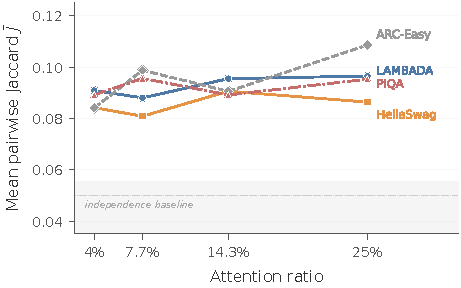
\includegraphics[width=\textwidth]{figures/fig4_jaccard_saturation.pdf}
\end{minipage}
\caption{Per-example overlap appears stable from minimal attention across benchmarks. (a,\,b) LAMBADA: cross-architecture $\sigma$ shows a non-significant decreasing trend at 1.3B (solid; Bonferroni-adjusted $p = .167$) but partially rebounds at 340M (dashed), while pairwise Jaccard of helped/hurt sets appears stable from 4\% attention onward. (c) This pattern holds across all four main benchmarks: mean pairwise $\bar{J}$ remains flat across attention ratios (all $\rho \leq 0.80$, $p \geq .333$). Shaded bands are illustrative ($n = 3$).}
\label{fig:decoupling}
\end{figure*}

This tension arises in the context of a rapid architectural shift toward hybrid recurrent-attention models, which interleave attention layers within linear recurrent backbones. Jamba \citep{lieber2024jamba}, Griffin \citep{de2024griffin}, RWKV-6 \citep{peng2024eagle}, and RecurrentGemma \citep{botev2024recurrentgemma} each combine recurrence with attention using different mixing strategies. These systems now serve as production-grade alternatives to pure Transformers, and the practical question of how much attention to include is typically answered by comparing aggregate benchmark numbers. \citet{wang2025hybrid} provide a controlled model zoo spanning three recurrent architectures, five attention ratios, and two parameter scales, which enables systematic study of how attention allocation affects these hybrid designs.

Prior work on predictive multiplicity \citep{marx2020predictive} and underspecification \citep{damour2022underspecification,mccoy2020berts} documents this risk for seed variation within a single architecture, but whether it extends to architectural variation in hybrid recurrent models remains open. If architectures that score similarly in aggregate behave differently on individual inputs, the backbone choice carries hidden consequences for deployment reliability and ensemble construction.

We present the first controlled within-family per-example analysis of how attention affects cross-architecture agreement in hybrid recurrent models. Using the model zoo of \citet{wang2025hybrid}, we compare three architectures (GatedDeltaNet, RetNet, HGRN2) at five attention ratios (0--25\%) and two scales (340M, 1.3B). We evaluate all 30 configurations on 10 benchmarks spanning retrieval, comprehension, reasoning, and mixed categories. On four benchmarks (LAMBADA \citealp{paperno2016lambada}, $N = 5{,}153$; HellaSwag \citealp{zellers2019hellaswag}, $N = 10{,}042$; PIQA \citealp{bisk2020piqa}, $N = 1{,}838$; ARC-Easy \citealp{clark2018arc}, $N = 2{,}376$) we conduct per-example decompositions, classifying each example as helped, hurt, or unchanged when attention is added, and measure cross-architecture overlap via Jaccard similarity. Figure~\ref{fig:decoupling} previews our central finding: architectures that appear equivalent by aggregate benchmarks diverge systematically at the per-example level, and this divergence is established by minimal attention.

Our central finding is that architectural variation produces structured predictive multiplicity whose magnitude depends on task type, not attention ratio. The ambiguity $\alpha$ (the fraction of examples on which the models disagree; \citealp{marx2020predictive}) ranges from 0.14 (PIQA) to 0.30 (LAMBADA), varies $2\times$ across task types but only 0.03 within each benchmark across attention ratios; pairwise Jaccard remains uniformly low ($\leq 0.14$, all $p < .01$ across all ten five-architecture pairs). A second finding is that per-example overlap appears to stabilize at the first attention level (4\%) and remains flat at higher ratios. Even on LAMBADA, where aggregate variance shows a non-significant decreasing trend ($\rho = -1.0$, Bonferroni-adjusted $p = .167$; at 1.3B only), per-example Jaccard does not change (\S\ref{ssec:decoupling}).

Our contributions are as follows:
\begin{itemize}
    \item Architectural variation in hybrid recurrent models, controlled within a single model zoo sharing training data and hyperparameters, produces structured predictive multiplicity whose magnitude varies by task type (or evaluation format) rather than attention ratio (\S\ref{ssec:per_example}). Five-architecture validation confirms the pattern (\S\ref{ssec:robustness}; Appendix~\ref{app:extended_arch}).
    \item Per-example overlap appears to stabilize at the first attention level (4\%) across all four benchmarks: minimal attention may establish which examples each architecture affects, with no observed homogenization at higher ratios ($n = 5$ ratios; \S\ref{ssec:decoupling}).
    \item Pure-model confidence margins partially predict which examples attention will affect (AUC 0.70--0.74), with rescue thresholds architecture-invariant but disruption thresholds varying 47\% across architectures, constituting a second dimension of multiplicity beyond per-example disagreement (\S\ref{ssec:per_example}; Appendix~\ref{app:prediction_framework}).
\end{itemize}


\section{Related Work}

\paragraph{Hybrid Recurrent Architectures.}
The design space for combining attention with recurrence spans layer-level interleaving \citep[Jamba;][]{lieber2024jamba}, local attention pairing \citep[Griffin, RecurrentGemma;][]{de2024griffin,botev2024recurrentgemma}, matrix-valued recurrence \citep[RWKV-6;][]{peng2024eagle}, within-head mixing \citep[Hymba;][]{dong2024hymba}, and unbounded-context hybrid SSMs \citep[Samba;][]{ren2024samba}. Mamba-2 \citep{dao2024mamba2} establishes a duality between structured state spaces and attention, while \citet{ali2025hidden} reveal implicit attention within Mamba. Comparative evaluations confirm that hybrids outperform pure Transformers and SSMs at scale \citep{waleffe2024empirical}, and that even one attention layer enables content-based routing \citep{basu2026routing}. Recent theoretical work establishes a provable expressiveness hierarchy between hybrid and pure linear attention \citep{ye2026provable}, providing formal grounding for the architectural differences we characterize at the per-example level. \citet{wang2025hybrid} provide the controlled model zoo we use, holding training conditions constant while varying architecture and attention ratio.

\paragraph{Linear Recurrent Models.}
Our three recurrent backbones represent distinct gating strategies within the linear recurrence family: RetNet \citep{sun2023retnet} uses multi-scale exponential decay, HGRN2 \citep{qin2024hgrn2} applies gated state expansion, and GatedDeltaNet \citep{yang2024gateddeltanet} combines gated updates with delta rules, extending GLA \citep{yang2024gla} and DeltaNet \citep{yang2024deltanet}. These descend from S4 \citep{gu2022s4} and Mamba \citep{gu2024mamba}, which introduced structured state spaces and input-dependent selection, and connect to linear attention \citep{katharopoulos2020transformers} through the state-space--attention duality of Mamba-2. xLSTM \citep{beck2024xlstm} revives the LSTM lineage with exponential gating and matrix memory, offering an alternative approach at scale. \citet{zimerman2025unified} show that modern gated-linear RNNs (including RetNet and HGRN) can all be cast as implicit causal self-attention, providing a unifying perspective on the family. \citet{arora2024based} identify a recall-throughput tradeoff in linear models that motivates hybrid designs.

\paragraph{Underspecification and Predictive Multiplicity.}
\citet{damour2022underspecification} formalized underspecification, where equivalent aggregate performance masks per-prediction divergence, with NLP instances including seed-dependent BERT disagreement \citep{mccoy2020berts,sellam2022multiberts}. \citet{marx2020predictive} introduced predictive multiplicity, showing that near-optimal models produce conflicting per-example predictions; extensions address probabilistic settings \citep{watson2023predictive}, Rashomon capacity \citep{hsu2022rashomon}, and reconciliation \citep{du2025reconciling,haghighat2026resolving}. These studies, along with Rashomon-set analyses \citep{fisher2019all,semenova2022existence} and weight-space interpolation \citep{wortsman2022model}, attribute divergence to initialization noise within a single architecture. We show that changing the recurrent backbone, a qualitatively different source of variation, produces per-example multiplicity that varies by task type. Our routing approach relates to selective prediction \citep{geifman2017selective} and ensemble selection \citep{caruana2004ensemble}, though we select among architecturally distinct models. \citet{yang2026benchmark} demonstrate analogous per-item disagreement (16--66\%) among frontier LLMs; our within-family design isolates backbone variation from training-regime differences.


\section{Method}\label{sec:method}

We describe the model configurations, evaluation benchmarks, and analytical framework used to measure how attention affects cross-architecture agreement at both aggregate and per-example levels.

\begin{table}[t]
\centering
\small
\caption{Model zoo summary \citep{wang2025hybrid}. All configurations share training data, tokenizer, and hyperparameters; they differ only in backbone and attention ratio.}
\label{tab:model_zoo}
\begin{tabular}{@{}lll@{}}
\toprule
Architecture & Recurrence mechanism & Scales \\
\midrule
GatedDeltaNet & Gated delta rules & 340M, 1.3B \\
RetNet & Multi-scale exp.\ decay & 340M, 1.3B \\
HGRN2 & Gated state expansion & 340M, 1.3B \\
\midrule
\multicolumn{3}{@{}l@{}}{\footnotesize Attention ratios: 0\%, 4\%, 7.7\%, 14.3\%, 25\%} \\
\multicolumn{3}{@{}l@{}}{\footnotesize Extended (340M only): +GLA, +DeltaNet} \\
\bottomrule
\end{tabular}
\end{table}

\subsection{Model Zoo}\label{ssec:model_zoo}

We use the pretrained model zoo of \citet{wang2025hybrid} (Table~\ref{tab:model_zoo}), which provides controlled comparisons: GatedDeltaNet (GDN; \citealp{yang2024gateddeltanet}), RetNet \citep{sun2023retnet}, and HGRN2 \citep{qin2024hgrn2} at five attention ratios and two scales. The GDN 1.3B h3-1 configuration uses 16 attention heads vs.\ 32 for RetNet and HGRN2 (\S\ref{ssec:robustness}). We adopt the h$k$-1 notation: h3-1 = 25\% attention, h6-1 = 14.3\%, h12-1 = 7.7\%, h24-1 = 4\%. Within each scale, all models share identical training data, tokenizer, and hyperparameters, isolating architecture and attention configuration. The zoo also includes a Transformer baseline at both scales.

\subsection{Task Taxonomy}\label{ssec:task_taxonomy}

We evaluate on 10 benchmarks grouped into four categories defined by the primary cognitive demand of each task. This taxonomy (informal; not pre-registered) was fixed prior to analysis following standard categorizations in the evaluation literature \citep{arora2024zoology} and is treated as hypothesis-generating rather than confirmatory (see Appendix~\ref{app:benchmark_details} for the confirmatory/exploratory split), not derived post hoc from observed results. The categories test whether the effect of attention on cross-architecture variance depends on task type.

\begin{itemize}
    \item \textbf{Retrieval}: LAMBADA \citep{paperno2016lambada}, which requires predicting a final word from long-range context without reasoning or world knowledge.
    \item \textbf{Comprehension}: BoolQ \citep{clark2019boolq}, a reading comprehension task with yes/no answers.
    \item \textbf{Reasoning}: HellaSwag \citep{zellers2019hellaswag}, ARC-Challenge \citep{clark2018arc}, WinoGrande \citep{sakaguchi2020winogrande}, and PIQA \citep{bisk2020piqa}. COPA \citep{roemmele2011copa} ($n = 100$) is supplementary; its small sample renders $\alpha$ unreliable (Appendix~\ref{app:subsample_sensitivity}).
    \item \textbf{Mixed}: ARC-Easy \citep{clark2018arc}, MMLU \citep{hendrycks2021mmlu}, SciQ \citep{welbl2017sciq}, and XStoryCloze \citep{lin2022xstorycloze}, which combine retrieval, comprehension, and reasoning demands.
\end{itemize}

LAMBADA is the only free-form generation benchmark in our evaluation; all others use multiple-choice scoring. Its higher $\alpha$ (0.30 vs.\ 0.14--0.21 for multiple-choice tasks) may partly reflect the larger answer space inherent to open-ended prediction, and the multiple-choice format may mechanically constrain per-example divergence by limiting the number of distinct error patterns. We cannot fully disentangle task type from evaluation format with the present benchmarks. However, within multiple-choice tasks, format (two-way vs.\ four-way) does not predict $\alpha$ (\S\ref{ssec:per_example}), suggesting that format alone does not drive the observed variation.

All evaluations use lm-evaluation-harness v0.4.x \citep{gao2024lmeval} with default prompts and greedy decoding; accuracy serves as the primary metric for all benchmarks. Bootstrap analyses use random seed 42 throughout.

\subsection{Convergence Metrics}\label{ssec:convergence_metrics}

We quantify cross-architecture agreement as a function of attention ratio. For each benchmark and attention ratio, we compute the cross-architecture standard deviation $\sigma$ over the three architectures' accuracy scores. To measure the relationship between attention and convergence, we compute the Spearman rank correlation $\rho$ between attention ratio rank and $\sigma$ across the five attention configurations ($n = 5$). A negative $\rho$ indicates that higher attention ratios are associated with lower cross-architecture variance.

We also report the convergence ratio $\sigma_{\text{pure}} / \sigma_{\text{h3-1}}$, defined as the standard deviation under the pure-recurrent configuration divided by that under the highest attention ratio (25\%). Values greater than 1 indicate that higher attention ratios are associated with lower cross-architecture variance.

\begin{figure}[t]
\centering
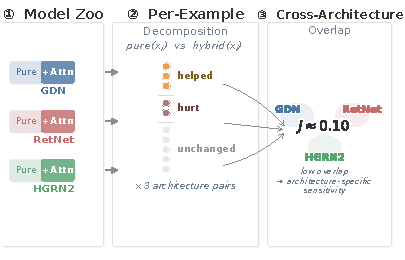
\includegraphics[width=\columnwidth]{figures/fig_method_overview.pdf}
\caption{Experimental framework. For each architecture, we compare the pure-recurrent baseline against its hybrid (+attention) variant, classifying every evaluation example as helped, hurt, or unchanged. Cross-architecture overlap of these per-example effect sets is measured via pairwise Jaccard similarity ($J \approx 0.10$), revealing architecture-specific sensitivity patterns.}
\label{fig:method_overview}
\end{figure}

\subsection{Per-Example Decomposition}\label{ssec:per_example_decomposition}

We decompose performance changes at the individual-example level on four benchmarks spanning three task categories: LAMBADA (5{,}153 examples; retrieval), HellaSwag (10{,}042; reasoning), PIQA (1{,}838; reasoning, two-choice), and ARC-Easy (2{,}376; mixed). HellaSwag uses normalized accuracy (acc\_norm) as the per-example correctness criterion. Supplementary analyses on BoolQ (3{,}270) and WinoGrande (1{,}267) appear in Appendix~\ref{app:boolq} and \ref{app:winogrande}. For each architecture, we compare the pure-recurrent baseline against its h3-1 hybrid (25\% attention), which maximizes the recurrent--hybrid contrast; \S\ref{ssec:per_example} confirms that $\alpha$ is stable across intermediate ratios (variation $< 0.03$). Each example is classified as:

\begin{itemize}
    \item \textbf{Helped}: correct in the hybrid but incorrect in the pure model.
    \item \textbf{Hurt}: correct in the pure model but incorrect in the hybrid.
    \item \textbf{Unchanged}: both models agree (both correct or both incorrect).
\end{itemize}

The net effect for each architecture is $|\text{helped}| - |\text{hurt}|$. A positive net effect means more examples transition to correct than to incorrect when attention is added; a negative net effect means the opposite.

To measure cross-architecture overlap, we compute the pairwise Jaccard similarity $J = |A \cap B| / |A \cup B|$ between the helped sets of two architectures and, separately, between their hurt sets. $J = 1$ indicates identical sets; $J = 0$ indicates no overlap. On $K$-choice tasks, binarization collapses $K{-}1$ wrong answers into a single ``incorrect'' category, potentially counting architectures as agreeing (both wrong) when they select different wrong answers. This conservative bias strengthens the multiplicity claim: true divergence may exceed what binary Jaccard captures. Appendix~\ref{app:continuous_jaccard} confirms robustness under continuous Jaccard similarity.

\subsection{Statistical Methods}\label{ssec:statistical_methods}

All tests are two-tailed. Spearman $\rho$ uses exact permutation tests ($5! = 120$ permutations); with $n = 5$, only $|\rho| = 1.0$ achieves $p < .05$ ($p = .017$), so all Spearman-based inferences are descriptive and exploratory. Bonferroni correction spans all 10 benchmarks (adjusted threshold $\alpha / 10 = 0.005$). Bootstrap 95\% bias-corrected and accelerated (BCa) confidence intervals use 10{,}000 resamples; with $n = 3$ architectures, these are heuristic indicators of effect direction. Within-architecture comparisons use Mann-Whitney U; cross-architecture comparisons use Kruskal-Wallis. Attention weight analysis extracts per-layer cosine similarity and Shannon entropy via forward hooks (Appendix~\ref{app:attention_patterns}). The permutation null does not condition on item difficulty; if difficulty-driven correlations inflate observed Jaccard while permutation destroys this structure, the test may be anti-conservative. However, the ${\sim}2\times$ observed-to-null ratio (all $z > 5.9$) provides substantial margin against this bias.

\begin{figure}[t]
\centering
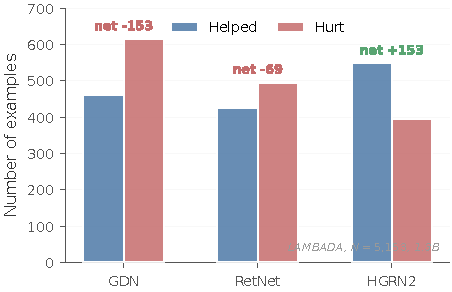
\includegraphics[width=\columnwidth]{figures/fig_per_example_bars.pdf}
\caption{Per-example effects of adding attention (pure $\to$ h3-1) on LAMBADA (1.3B). Helped: correct only with attention; hurt: correct only without. HGRN2 shows the only net positive effect; overlap is minimal ($\bar{J} \leq 0.10$, all $p < .0001$).}
\label{fig:per_example_bars}
\end{figure}


\section{Experiments}\label{sec:experiments}

Using the model zoo of \citet{wang2025hybrid} (\S\ref{ssec:model_zoo}), we evaluate all 30 configurations on 10 benchmarks plus supplementary COPA ($n = 100$) at 1.3B scale unless noted. Results at 340M appear in scale analyses. Recall: h$k$-1 denotes one attention layer per $k{+}1$ layers; h3-1 = 25\% attention.

\subsection{Per-Example Divergence}\label{ssec:per_example}

Do architectures converge by improving on the same examples? We compare each architecture's pure-recurrent baseline against its h3-1 hybrid on 5{,}153 LAMBADA examples, classifying each as helped, hurt, or unchanged. Although the decomposition is binary, it captures genuine separation in the continuous confidence space (Cohen's $d = 0.73$--$0.92$ between helped and hurt on LAMBADA; cross-benchmark details in Appendix~\ref{app:cm_cross}). Binarization discards confidence magnitude, so we supplement with continuous confidence margin analysis (Appendix~\ref{app:confidence_margin}) and verify that low Jaccard persists under continuous thresholds (Appendix~\ref{app:continuous_jaccard}).

\begin{figure}[t]
\centering
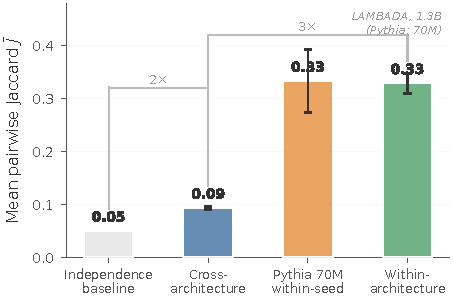
\includegraphics[width=\columnwidth]{figures/fig_jaccard_hierarchy.pdf}
\caption{Jaccard hierarchy on LAMBADA (1.3B). Cross-architecture overlap ($\bar{J} \approx 0.09$) is $2\times$ the independence baseline but only one-third of within-architecture overlap ($\bar{J} \approx 0.33$). Pythia 70M within-seed Jaccard (different scale) falls at a comparable level. Error bars show the helped--hurt range.}
\label{fig:jaccard_hierarchy}
\end{figure}

\begin{figure*}[t]
\centering
\includegraphics[width=0.75\textwidth]{figures/fig3_alpha_routing.pdf}
\caption{(a) Per-example ambiguity $\alpha$ varies $2\times$ across task types. (b) Confidence-based routing gains track $\alpha$: effective when multiplicity is high (LAMBADA) but counterproductive when low (PIQA). 1.3B, h3-1.}
\label{fig:alpha_routing}
\end{figure*}

Each architecture displays a distinct profile of per-example changes (Figure~\ref{fig:per_example_bars}). GDN loses a net 153 examples (462 helped, 615 hurt), RetNet loses 69 (426/495), and HGRN2 gains 153 (548/395; full counts in Appendix~\ref{app:per_example_counts}). HGRN2 is the only architecture for which adding attention yields a net per-example benefit. Pairwise Jaccard similarity is low: mean $\bar{J} \leq 0.10$, indicating ${\sim}90$\% non-overlap. Overlap significantly exceeds the independence baseline ($J_{\text{null}} \approx 0.05$, all $z > 5.9$, $p < .0001$; Appendix~\ref{app:jaccard_permutation}), plausibly reflecting shared sensitivity to example difficulty. Normalizing by $J_{\max}$, observed overlap reaches only 6--7\% of the achievable range above chance (Appendix~\ref{app:normalized_es}), confirming that low Jaccard cannot be attributed to set-size constraints.


\paragraph{Confidence margin predictor.} Pure-model confidence on the target token predicts which examples will be affected (AUC 0.70--0.74, a non-parametric measure equivalent to Mann-Whitney $U$; Appendix~\ref{app:confidence_margin}): rescue thresholds (the confidence below which wrong answers are likely corrected by attention) are architecture-invariant (1\% spread) but disruption thresholds (the confidence above which correct answers become vulnerable) vary 47\%, explaining cross-architecture Jaccard divergence (Appendix~\ref{app:prediction_framework}). Calibration differences account for less than half the threshold spread (Appendix~\ref{app:calibration}). The rescue pattern generalizes across three benchmarks ($d = 0.13$--$0.60$; Appendix~\ref{app:cm_cross}); disruption is weaker on reasoning tasks (Appendix~\ref{app:boolq}). This structured disagreement constitutes predictive multiplicity \citep{marx2020predictive} under architectural variation.

\paragraph{Confidence-based routing.} As an illustrative case study, the rescue-threshold asymmetry suggests a routing strategy: select the architecture whose pure-model confidence best predicts successful rescue. On LAMBADA, this outperforms majority vote by $+5.3$\,pp (SD $= 0.4$\,pp, 10 cross-validated splits), extracting 36\% of the oracle gap (oracle = 65.5\%; Appendix~\ref{app:complementarity}). On ARC-Easy, gains are modest ($+1.0$\,pp, SD $= 0.5$\,pp); on HellaSwag, routing provides no benefit ($-0.02$\,pp, $p = .89$); on PIQA, it is significantly negative ($-0.6$\,pp, $p = .006$). Routing works when multiplicity is high ($\alpha = 0.30$, LAMBADA) and a clear rescue-threshold signal exists, but is counterproductive when multiplicity is low ($\alpha = 0.14$, PIQA). A natural comparison (average-logits ensemble) is left to future work as it requires simultaneous inference across all architectures.

\paragraph{Complementarity structure.} Table~\ref{tab:complementarity} decomposes the three-architecture vote on each example. On LAMBADA, 15.1\% of examples are majority-exploitable (2/3 correct) and 14.5\% are majority-hostile (1/3 correct)---a near-even split yielding a majority-vote exploitation ratio of only ${\sim}51$\%. The oracle exploits both categories, explaining the large oracle--MV gap ($+14$\,pp on LAMBADA). This structural constraint is stable across attention ratios (51--54\% on LAMBADA across all five configurations; Appendix~\ref{app:complementarity}).

\begin{table}[t]
\centering
\small
\caption{Complementarity decomposition at 1.3B h3-1. Fractions of examples where $k$ of 3 architectures answer correctly. MV expl.: fraction of non-unanimous examples where majority vote is correct.}
\label{tab:complementarity}
\begin{tabular}{@{}lccccr@{}}
\toprule
Benchmark & 3/3 & 2/3 & 1/3 & 0/3 & MV expl. \\
\midrule
LAMBADA & .361 & .151 & .145 & .343 & 51.1\% \\
HellaSwag & .519 & .078 & .073 & .331 & 51.6\% \\
ARC-Easy & .603 & .107 & .103 & .187 & 50.9\% \\
\bottomrule
\end{tabular}
\end{table}

\paragraph{Multiplicity variation.} Extending to HellaSwag ($N = 10{,}042$) and PIQA ($N = 1{,}838$) reveals that multiplicity varies systematically across tasks (Table~\ref{tab:multiplicity}). Ambiguity $\alpha$ \citep{marx2020predictive} ranges from 0.14 (PIQA) through 0.15 (HellaSwag) and 0.21 (ARC-Easy; Appendix~\ref{app:arceasy}) to 0.30 (LAMBADA). Format does not drive this ordering: HellaSwag (four-way) and PIQA (two-choice) produce nearly identical $\alpha$ despite different answer-space sizes ($\rho = -0.60$, $p = .24$ with task accuracy). This suggests multiplicity is associated with cognitive demands rather than evaluation format, though the confound cannot be fully resolved (Limitations). Bootstrap 95\% CIs confirm the ordering (all non-overlapping except PIQA--HellaSwag; Table~\ref{tab:arceasy_ambiguity}). Pairwise Jaccard remains uniformly low ($\bar{J} \leq 0.10$, all $p < .01$), indicating architectures affect different examples regardless of how many are affected. Within each benchmark, $\alpha$ is stable across attention ratios (variation $< 0.03$) but differs $2\times$ across task types, confirming that multiplicity magnitude depends on task, not attention ratio \citep[cf.][]{gorbett2026crossmodel}.

\begin{figure}[t]
\centering
\includegraphics[width=\columnwidth]{figures/fig2_task_specificity.pdf}
\caption{Spearman $\rho$ between attention ratio and cross-architecture $\sigma$ for each benchmark at 1.3B scale. LAMBADA ($\rho = -1.0$; BCa 95\% CI $[-1.0,\,-0.7]$, heuristic) is the only benchmark whose CI excludes zero. Bootstrap CI is heuristic given $n = 3$ architectures.}
\label{fig:task_specificity}
\end{figure}

\begin{figure*}[t]
\centering
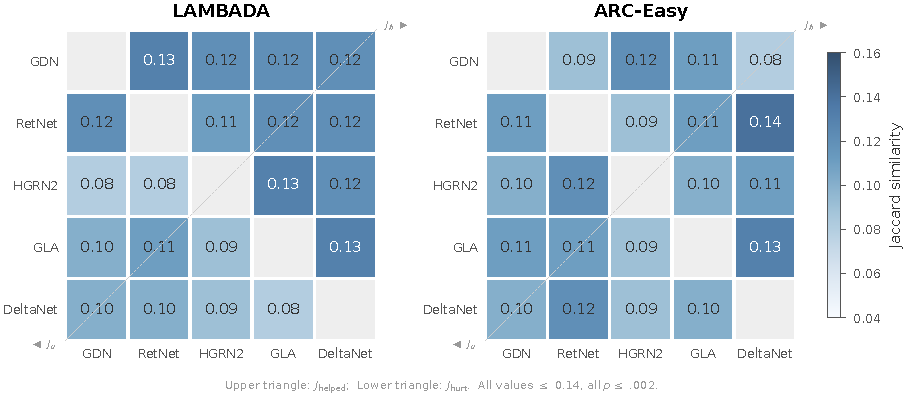
\includegraphics[width=0.75\textwidth]{figures/jaccard_heatmap_5arch.pdf}
\caption{Pairwise Jaccard heatmap across five architectures (340M, h3-1), where helped (hurt) examples are those correct only with (without) attention. Upper triangle: $J_{\text{helped}}$; lower triangle: $J_{\text{hurt}}$. All values $\leq 0.14$, all permutation tests $p < .005$. HellaSwag and PIQA results in Appendix~\ref{app:extended_arch}.}
\label{fig:jaccard_heatmap_5arch}
\end{figure*}

\begin{table}[t]
\centering
\small
\caption{Predictive multiplicity at 1.3B, h3-1. $\alpha$: ambiguity \citep{marx2020predictive}; $\bar{J}$: mean pairwise Jaccard of helped~(h) / hurt~(u) sets; $\rho_\alpha$: Spearman $\rho$ of $\alpha$ vs.\ attention ratio.}
\label{tab:multiplicity}
\vspace{1pt}
\begin{tabular}{@{}lrcccc@{}}
\toprule
 & $N$ & $\alpha$ & $\bar{J}_{h}$ & $\bar{J}_{u}$ & $\rho_\alpha$ \\
\midrule
PIQA & 1838 & .14 & .091 & .094 & $0.0$ \\
HellaSwag & 10042 & .15 & .095 & .085 & $0.1$ \\
ARC-Easy & 2376 & .21 & .092 & .099 & $-0.2$ \\
LAMBADA & 5153 & .30 & .100 & .093 & $-0.6$ \\
\bottomrule
\end{tabular}
\par\vspace{2pt}
{\footnotesize Within-benchmark $\alpha$ variation $< 0.03$ across ratios. BoolQ, WinoGrande: Appendix~\ref{app:boolq}, \ref{app:winogrande}.}
\vspace{-4pt}
\end{table}

\begin{table}[t]
\centering
\caption{Cross-architecture variance trends across benchmarks (1.3B scale). $\rho$: Spearman correlation between attention ratio and cross-architecture $\sigma$ across five configurations. $p$: exact permutation test (two-tailed). $\sigma$ values $\times 10^{2}$ (accuracy pp). Ratio: $\sigma_{\text{pure}} / \sigma_{\text{h3-1}}$. \textbf{Bold}: only benchmark with $\rho = -1.0$.}
\label{tab:convergence}
\footnotesize
\setlength{\tabcolsep}{2.5pt}
\begin{tabular}{@{}llrrrrr@{}}
\toprule
Benchmark & Cat.\ & $\rho$ & $p$ & $\sigma_{\text{p}}$ & $\sigma_{\text{h3}}$ & Ratio \\
\midrule
\textbf{LAMBADA$^{\ddagger}$} & \textbf{Ret.} & $\mathbf{-1.0}$ & \textbf{.017} & \textbf{2.41} & \textbf{0.49} & \textbf{4.87} \\
\quad\emph{(excl.\ GDN)} & & $-0.7$ & .233 & --- & --- & --- \\
BoolQ & Comp. & $0.2$ & .783 & 1.63 & 2.36 & 0.69 \\
ARC-C & Reas. & $0.6$ & .350 & 0.96 & 1.32 & 0.72 \\
HellaSwag & Reas. & $0.3$ & .683 & 1.17 & 1.18 & 0.99 \\
PIQA & Reas. & $-0.5$ & .450 & 0.54 & 0.34 & 1.59 \\
WinoGrande & Reas. & $0.1$ & .950 & 0.67 & 0.78 & 0.86 \\
ARC-E & Mix. & $-0.7$ & .233 & 1.00 & 0.13 & 7.70 \\
MMLU & Mix. & $-0.7$ & .233 & 0.92 & 0.41 & 2.27 \\
SciQ & Mix. & $0.1$ & .950 & 0.87 & 0.74 & 1.19 \\
XStoryCloze & Mix. & $-0.6$ & .350 & 0.82 & 0.55 & 1.49 \\
\midrule
COPA$^{\dagger}$ & Reas. & $-0.67$ & .267 & 2.63 & 0.47 & 5.57 \\
\bottomrule
\multicolumn{7}{l}{\scriptsize $^{\dagger}$Supplementary ($n = 100$); excl.\ from multiple comparison corr.} \\
\multicolumn{7}{l}{\scriptsize $^{\ddagger}$GDN h3-1: 16 attn heads; others use 32 (\S\ref{ssec:robustness}).} \\
\multicolumn{7}{@{}p{\columnwidth}@{}}{\scriptsize Bonf.-adj.\ $p = .167$. \textbf{Only $|\rho| = 1.0$ achieves $p < .05$ at $n = 5$.} Excl.\ GDN reverses MMLU $\rho$ to $+0.6$ (\S\ref{ssec:robustness}). HellaSwag uses acc\_norm.}
\end{tabular}
\vspace{-4pt}
\end{table}

\subsection{Per-Example Overlap Appears Stable from Minimal Attention}\label{ssec:decoupling}

Having established that multiplicity varies by task type, we now ask whether it changes with the amount of attention. Does adding more attention change \emph{which} examples each architecture affects? Pairwise Jaccard appears to stabilize at the first attention level (4\%; $\bar{J} \approx 0.095$) and remains flat across all higher ratios (Figure~\ref{fig:decoupling}b), suggesting that minimal attention may suffice to establish the per-example divergence pattern, though the small number of ratios ($n = 5$) limits statistical confirmation. As background, LAMBADA's aggregate cross-architecture $\sigma$ shows a non-significant decreasing trend ($\rho = -1.0$, Bonferroni-adjusted $p = .167$; excluding GDN: $\rho = -0.7$, $p = .233$; MMLU reverses to $\rho = +0.6$ when excluding GDN; observed at 1.3B, absent at 340M; Table~\ref{tab:convergence}, Figure~\ref{fig:task_specificity}). No other benchmark shows a comparable aggregate pattern ($n = 5$; negligible power for $|\rho| < 1.0$; Appendix~\ref{app:convergence_detail}).


Each architecture's per-example response is largely idiosyncratic: observed $\bar{J}$ reaches only 6--7\% of the achievable range above chance ($J_{\max} \approx 0.78$--$0.92$), ruling out ceiling constraints (\S\ref{ssec:per_example}). This pattern generalizes beyond LAMBADA (Figure~\ref{fig:decoupling}c): on all four main benchmarks, mean pairwise Jaccard shows no significant trend with attention ratio (all $\rho \leq 0.80$, $p \geq 0.333$; Appendix~\ref{app:cross_bench_jaccard}).

Heuristic bootstrap 95\% CIs ($n = 3$; \S\ref{ssec:statistical_methods}) show non-overlapping $\sigma$ between pure and h3-1 but completely overlapping Jaccard across all hybrid ratios. Figure~\ref{fig:jaccard_hierarchy} shows a three-tier Jaccard hierarchy: independence baseline (${\sim}0.05$), cross-architecture (${\sim}0.10$, $2\times$ baseline), and within-architecture (${\sim}0.33$, $3\times$ cross-architecture; Appendix~\ref{app:within_arch_stability}). Pythia 70M \citep{biderman2023pythia} seed calibration yields a comparable within-seed level ($J = 0.27$--$0.39$; Appendix~\ref{app:seed_calibration}), consistent with architecture-associated divergence.

Two interpretations are consistent with the observed stability. \textbf{(a) Fingerprint view:} each recurrent backbone imposes a characteristic inductive bias that determines which examples attention can rescue. \textbf{(b) Convergence view:} even minimal attention causes all architectures to rapidly adopt Transformer-like behavior, with residual divergence from incomplete convergence.

\begin{table}[t]
\centering
\small
\caption{Transformer entrainment: Jaccard similarity between each model's correct set and a Transformer baseline on LAMBADA (1.3B). All h3-1 hybrids shift toward the Transformer pattern; the Transformer itself scores lowest (48.1\%), so the shift is not explained by degradation.}
\label{tab:entrainment}
\begin{tabular}{@{}lccc@{}}
\toprule
Architecture & $J_{\text{pure,T}}$ & $J_{\text{h3-1,T}}$ & $\Delta$ \\
\midrule
GDN & 0.645 & 0.649 & $+$0.005 \\
RetNet & 0.679 & 0.694 & $+$0.015 \\
HGRN2 & 0.672 & 0.701 & $+$0.029 \\
\bottomrule
\end{tabular}
\end{table}

Table~\ref{tab:entrainment} provides partial support for interpretation~(b): all three h3-1 hybrids' correct sets are more similar to a Transformer baseline than their pure-recurrent counterparts. The shift is strongest for HGRN2 ($\Delta = +0.029$), the only architecture with a net positive per-example effect, suggesting that architectures which benefit most from attention also converge most toward Transformer-like behavior.

However, attention weight analysis complicates a pure convergence account: at 1.3B h3-1, GDN and RetNet produce nearly identical mean attention distributions (cosine 0.995; Appendix~\ref{app:attention_patterns}), yet their per-example effect sets overlap by only $J \approx 0.10$. The dissociation points to the recurrent layers as the primary source of multiplicity: the same attention signal, processed through different recurrent substrates, yields architecture-specific per-example outcomes.

Cross-scale analysis reveals a clear dissociation: per-example Jaccard is consistent across scales ($\bar{J} = 0.08$--$0.10$ at 340M and 1.3B), whereas the aggregate variance trend is observed only at 1.3B on LAMBADA ($\rho = -0.50$, $p = .45$ at 340M). Ambiguity $\alpha$ is systematically higher at 340M ($\Delta \leq 8$\,pp), suggesting the \emph{pattern} of multiplicity is scale-stable while its magnitude tracks model capacity (Appendices~\ref{app:scale_convergence}, \ref{app:scale_per_example}--\ref{app:cross_scale}).
\vspace{-2pt}
\subsection{Robustness}\label{ssec:robustness}

Removing GDN weakens the LAMBADA variance reduction ($\rho = -0.7$, $p = .233$) and reverses MMLU's ($\rho = +0.6$), both driven by GDN's 16-head configuration (vs.\ 32 in others; Appendix~\ref{app:gdn_confound}). The RetNet--HGRN2 pair preserves the independence pattern ($\sigma \leq 0.008$, $J = 0.086$--$0.108$). The aggregate variance pattern therefore depends on GDN inclusion; the per-example stability pattern does not. Five-architecture validation at 340M (adding GLA and DeltaNet) confirms $J \leq 0.14$ across all ten pairwise comparisons and four benchmarks (all $p < .01$; Figure~\ref{fig:jaccard_heatmap_5arch}; Appendix~\ref{app:extended_arch}), extending the per-example divergence finding to architectures not used in the primary analysis. Full sensitivity analyses appear in Appendix~\ref{app:sensitivity}; Transformer baseline comparison in Appendix~\ref{app:transformer_entrainment}.


\section{Discussion and Conclusion}\label{sec:discussion}

When aggregate benchmarks show equivalent performance, the choice among hybrid architectures is often driven by efficiency considerations. Per-example multiplicity reveals a complementary dimension: each backbone handles a different subset of inputs correctly, determined by the recurrent mechanism rather than the attention configuration (\S\ref{ssec:decoupling}). For deployment contexts where per-example reliability matters, aggregate equivalence provides incomplete assurance. The complementarity structure (Table~\ref{tab:complementarity}) shows that oracle-level combination yields $+7$--$14$\,pp gains, but majority vote captures only ${\sim}51$\% because majority-exploitable and majority-hostile disagreements occur in near-equal proportion, motivating architecture-aware routing beyond simple ensembling. Our within-family design isolates backbone variation as the source of this multiplicity; \citet{yang2026benchmark} document analogous per-item disagreement (16--66\%) among frontier LLMs under conflated training regimes, suggesting the phenomenon is partly architectural in origin and resists homogenization even at minimal attention ratios.


\section*{Limitations}

Each configuration is a single training run; consistency across all 40 architecture--benchmark combinations mitigates but cannot fully resolve seed confounds.
We examine three architectures (plus two extended) from one model zoo at two scales; generalization to other hybrid families (Mamba, RWKV), larger scales (7B+), and open-ended generation remains open.
All evaluations use pretrained checkpoints with greedy decoding; per-example effects may not persist after fine-tuning or under alternative sampling strategies.

\bibliography{references}

\appendix
% Appendix sections for the paper.

\section{Confirmatory and Exploratory Analyses}\label{app:benchmark_details}

The task taxonomy used in \S\ref{ssec:task_taxonomy} was defined prior to running any convergence analyses. Each benchmark was assigned to exactly one of four categories based on the primary cognitive demand of the task:

\begin{itemize}
    \item \textbf{Retrieval}: tasks requiring prediction from long-range context without multi-step reasoning (LAMBADA).
    \item \textbf{Comprehension}: reading comprehension with explicit passage support (BoolQ).
    \item \textbf{Reasoning}: tasks requiring commonsense inference or multi-step reasoning (HellaSwag, ARC-Challenge, WinoGrande, PIQA).
    \item \textbf{Mixed}: tasks combining retrieval, comprehension, and reasoning demands (ARC-Easy, MMLU, SciQ, XStoryCloze).
\end{itemize}

\paragraph{Confirmatory benchmark set.} Six benchmarks were designated as confirmatory for Bonferroni correction: LAMBADA, HellaSwag, ARC-Challenge, WinoGrande, ARC-Easy, and MMLU. These were selected as representative of retrieval, reasoning, and mixed categories before any convergence analysis was performed. The taxonomy and benchmark selection were fixed before analysis as an informal pre-analysis plan; we describe this as a confirmatory/exploratory split rather than a formal pre-registration, since no external timestamp exists. The main text applies the more conservative all-10-benchmark correction (Bonferroni-adjusted $p = .017 \times 10 = .167$). \textbf{Sensitivity:} correcting across only the six confirmatory benchmarks yields adjusted $p = .017 \times 6 = .100$, still above conventional significance.

\paragraph{One-sided test.} If one adopts the prior that attention should reduce cross-architecture variance, the one-sided permutation $p$-value for LAMBADA is $1/120 \approx 0.0083$. Under 10-benchmark Bonferroni correction, this yields an adjusted $p = 0.083$, above the conventional threshold. We report two-sided tests throughout the main text as the more conservative choice; the one-sided result is noted here for completeness.

\paragraph{Exploratory benchmarks.} Four additional benchmarks (BoolQ, PIQA, SciQ, XStoryCloze) were added as exploratory tests. All benchmarks share the same 10-benchmark correction (adjusted threshold $\alpha / 10 = 0.005$) and the four exploratory benchmarks are labeled as such throughout the paper. The all-10 Bonferroni correction reported in the main text is the only correction used for inference; the exploratory 6-benchmark subset correction in this appendix is provided for transparency.

\paragraph{Supplementary benchmark.} COPA ($n = 100$) is treated as supplementary due to its small sample size. It is excluded from both correction families and reported separately with the $\dagger$ annotation in Table~\ref{tab:convergence}.

\section{Convergence Detail}\label{app:convergence_detail}

% Figure moved to main text (\S\ref{ssec:decoupling}).

Beyond LAMBADA ($\rho = -1.0$), two benchmarks show moderate negative correlations that do not reach significance: ARC-Easy and MMLU (both $\rho = -0.7$, $p = .233$). Both are classified as ``Mixed'' tasks combining retrieval with reasoning demands. The sensitivity analysis (Appendix~\ref{app:sensitivity}) shows that MMLU's correlation reverses upon GDN exclusion ($\rho = +0.6$), indicating dependence on a single architecture; ARC-Easy's correlation is more stable. COPA ($n = 100$; supplementary) shows $\rho = -0.67$ with a large $\sigma$ ratio (5.57), consistent with LAMBADA's pattern but unreliable due to small sample size.

Several benchmarks show positive or near-zero $\rho$ (BoolQ: $+0.2$; ARC-C: $+0.6$; HellaSwag: $+0.3$; WinoGrande: $+0.1$; SciQ: $+0.1$), indicating that attention does not systematically reduce cross-architecture variance on reasoning or comprehension tasks. The contrast with LAMBADA is consistent with attention's convergence benefit being specific to tasks requiring direct token-level recall \citep{arora2024zoology,arora2024based} rather than multi-step inference.

\paragraph{Regression to the mean.} The direction of LAMBADA's aggregate convergence is consistent with regression to the mean: GDN (highest pure accuracy, 0.543) declines to 0.513 under h3-1, while HGRN2 (lowest, 0.484) rises to 0.514, yielding a ${\sim}5\times$ $\sigma$ compression ($0.024 \to 0.005$). However, three observations argue against a purely statistical artifact. First, the ${\sim}5\times$ reduction in cross-architecture $\sigma$ far exceeds typical regression amplitudes. Second, the direction is entirely determined by architecture identity, not random fluctuation: HGRN2 accuracy increases monotonically across all attention ratios, while GDN decreases monotonically---a pattern inconsistent with noise-driven mean reversion. Third, per-example analysis (\S\ref{ssec:per_example}) reveals architecture-specific patterns: GDN's net $-153$ examples and HGRN2's net $+153$ examples reflect distinct helped/hurt profiles with low cross-architecture Jaccard overlap, indicating that the aggregate convergence arises from structured, architecture-dependent per-example changes rather than symmetric regression.

\section{Scale-Dependent Convergence}\label{app:scale_convergence}

At 1.3B parameters, LAMBADA convergence is monotonic: $\sigma$ decreases at every attention level from 0\% through 25\% ($\rho = -1.0$). At 340M, convergence is partial: $\sigma$ reaches a maximum reduction of 56\% at intermediate attention ratios but rebounds at h3-1, yielding a net endpoint reduction of 36\%. The trajectory is non-monotonic, and the highest-attention model does not achieve the lowest cross-architecture variance. One possible interpretation is that at smaller scale, the capacity overhead of attention layers creates interference that offsets the retrieval benefit.

This contrast is a preliminary observation from two data points (not a scaling law). Despite the aggregate divergence at 340M, mean pairwise Jaccard is similar at both scales ($J \approx 0.09$), extending the decoupling observation (\S\ref{ssec:decoupling}) to the scale dimension.

\section{Sensitivity Analyses}\label{app:sensitivity}

\subsection{Bootstrap Confidence Intervals}

We construct 95\% bootstrap confidence intervals for the Spearman $\rho$ between attention ratio and cross-architecture $\sigma$ on LAMBADA using 10{,}000 resamples at the architecture level ($n = 3$ architectures). Of these resamples, 11.25\% are degenerate: they consist of same-architecture triplicates, which produce a constant $\sigma$ vector and therefore an undefined $\rho$ (division by zero in the rank correlation formula). These are excluded from the confidence interval computation because they carry no information about the correlation, not because they represent $\rho = 0$.

The BCa (bias-corrected and accelerated) correction degenerates at the $\rho = -1.0$ boundary because the acceleration parameter requires finite jackknife variance, which collapses when the point estimate is at the distributional limit. We therefore report percentile confidence intervals instead. From the 88.75\% informative resamples, the 95\% percentile CI is $[-1.0,\,-0.7]$, which excludes zero.

\subsection{GDN Exclusion Sensitivity}

The GDN h3-1 configuration uses 16 attention heads rather than 32 (see Appendix~\ref{app:gdn_confound}). To assess the influence of this confound, we recompute all convergence correlations after excluding GDN, leaving two architectures (RetNet, HGRN2) at five attention ratios.

Table~\ref{tab:gdn_sensitivity} reports the results for benchmarks where the correlation changes by $|\Delta\rho| \geq 0.3$. LAMBADA weakens from $\rho = -1.0$ to $\rho = -0.7$ ($p = .233$), consistent with GDN contributing to the convergence signal. MMLU reverses from $\rho = -0.7$ to $\rho = +0.6$, confirming that the moderate negative correlation on MMLU depends on GDN's inclusion and should not be interpreted as evidence of convergence.

\begin{table}[ht]
\centering
\small
\caption{Effect of GDN exclusion on Spearman $\rho$ (attention ratio vs.\ cross-architecture $\sigma$) at 1.3B scale. Only benchmarks with $|\Delta\rho| \geq 0.3$ shown.}
\label{tab:gdn_sensitivity}
\begin{tabular}{lrrrr}
\toprule
Benchmark & $\rho_{\text{all}}$ & $\rho_{\text{no-GDN}}$ & $\Delta\rho$ & $p_{\text{no-GDN}}$ \\
\midrule
LAMBADA & $-1.0$ & $-0.7$ & $+0.3$ & .233 \\
MMLU & $-0.7$ & $+0.6$ & $+1.3$ & .350 \\
\bottomrule
\end{tabular}
\end{table}

\section{GDN Attention Head Confound}\label{app:gdn_confound}

In the \citet{wang2025hybrid} model zoo, the GDN h3-1 configuration at 1.3B scale uses 16 attention heads per attention layer, while all other hybrid configurations (across GDN, RetNet, and HGRN2) use 32 attention heads. This is a design choice in the original model zoo, not an error. The reduced head count changes the per-head dimension and may affect the attention capacity of GDN h3-1 relative to other configurations.

This confound is relevant because the convergence analysis measures cross-architecture $\sigma$ at each attention ratio. At the h3-1 ratio (25\% attention), GDN's attention layers have a different internal structure than those of RetNet and HGRN2, which could contribute to variance reduction (or inflation) for reasons unrelated to the recurrent--attention interaction under study.

The sensitivity analysis in Appendix~\ref{app:sensitivity} shows that removing GDN weakens the LAMBADA convergence correlation from $\rho = -1.0$ to $\rho = -0.7$. This weakening is partially attributable to the reduced sample size ($n = 2$ architectures) and partially to the confound itself. We cannot separate these two effects with the available data.

\section{Attention Weight Analysis}\label{app:attention_patterns}

We extract attention weight matrices from the 1.3B h3-1 models of all three architectures using forward hooks on each attention layer. While \citet{ali2025hidden} show that SSM layers learn implicit attention patterns, our analysis focuses on the explicit attention layers interleaved within the hybrid architecture. For each layer, we compute the mean attention distribution across all 5{,}153 LAMBADA examples and measure cross-architecture similarity via cosine similarity.

\subsection{Cross-Architecture Cosine Similarity}

Table~\ref{tab:attn_cosine} reports cosine similarity between mean attention distributions at selected layers and averaged across all layers.

\begin{table}[ht]
\centering
\caption{Cosine similarity between mean attention weight distributions of architecture pairs at selected layers (1.3B h3-1 models on LAMBADA).}
\label{tab:attn_cosine}
\resizebox{\columnwidth}{!}{%
\begin{tabular}{lrrr}
\toprule
Layer & GDN--RetNet & GDN--HGRN2 & HGRN2--RetNet \\
\midrule
L2 (early) & 0.995 & 0.244 & 0.196 \\
L20 (deep) & 0.986 & 0.942 & 0.943 \\
\midrule
Mean (all layers) & 0.905 & 0.766 & 0.698 \\
\bottomrule
\end{tabular}%
}
\end{table}

At layer 2, GDN and RetNet produce nearly identical attention distributions (cosine 0.995), while HGRN2 diverges from both (cosine $< 0.25$). By layer 20, all three architectures converge to similar attention patterns (cosine $> 0.94$). The layer-wise trajectory suggests that early-layer attention patterns are shaped by the preceding recurrent layers (which differ across architectures), while deeper layers converge regardless of the recurrent substrate.

\subsection{Helped vs.\ Hurt Attention Entropy}

To test whether the attention mechanism itself differs between helped and hurt examples, we compute the Shannon entropy of the attention distribution for each example at each attention layer and compare the mean entropy of helped examples against hurt examples within each architecture.

\begin{table}[ht]
\centering
\caption{Mean attention entropy difference (helped $-$ hurt) averaged across attention layers (1.3B h3-1 models on LAMBADA). Values near zero indicate that the attention mechanism does not discriminate between helped and hurt examples.}
\label{tab:attn_entropy}
\begin{tabular}{lr}
\toprule
Architecture & $\Delta H$ (helped $-$ hurt) \\
\midrule
GDN & $-0.0009$ \\
RetNet & $+0.0179$ \\
HGRN2 & $+0.0020$ \\
\bottomrule
\end{tabular}
\end{table}

GDN and HGRN2 show negligible entropy differences ($|\Delta H| \leq 0.002$). RetNet's $\Delta H = +0.018$ is small in absolute terms but slightly larger; helped examples receive marginally more diffuse attention in RetNet. Across all three architectures, the differences are insufficient to explain the per-example divergence, consistent with per-example effects not being explained by attention weight patterns and likely originating in the recurrent layers.

\subsection{Last-5 Attention Mass}

We also measure the fraction of attention mass allocated to the last five tokens, which captures whether the attention mechanism concentrates differently on recent context for helped vs.\ hurt examples.

\begin{table}[ht]
\centering
\caption{Mean attention mass on last-5 tokens for helped and hurt examples, averaged across attention layers (1.3B h3-1 models on LAMBADA).}
\label{tab:attn_last5}
\begin{tabular}{lrr}
\toprule
Architecture & Helped & Hurt \\
\midrule
GDN & 0.0834 & 0.0831 \\
RetNet & 0.1578 & 0.1591 \\
HGRN2 & 0.0453 & 0.0467 \\
\bottomrule
\end{tabular}
\end{table}

No architecture shows a meaningful difference in last-5 attention mass between helped and hurt examples (Table~\ref{tab:attn_last5}). This further supports the conclusion that the per-example divergence is not driven by differential attention allocation.

\section{Cross-Scale Per-Example Comparisons}\label{app:cross_scale}

\subsection{Within-Scale Pairwise Jaccard}

Table~\ref{tab:within_scale_jaccard} reports the within-scale pairwise Jaccard similarity between architectures' helped and hurt sets at both scales. Mean values are similar across scales (340M: 0.094/0.090; 1.3B: 0.100/0.093), indicating that per-example architecture specificity is consistent across the two scales examined.

\begin{table}[ht]
\centering
\small
\caption{Within-scale pairwise Jaccard similarity of per-example effects (pure $\to$ h3-1) on LAMBADA. Each row compares the helped (or hurt) sets of two architectures at the same scale.}
\label{tab:within_scale_jaccard}
\begin{tabular}{llcc}
\toprule
Scale & Pair & $J_{\text{helped}}$ & $J_{\text{hurt}}$ \\
\midrule
\multirow{4}{*}{340M} & GDN--RetNet & 0.092 & 0.109 \\
& GDN--HGRN2 & 0.084 & 0.075 \\
& RetNet--HGRN2 & 0.108 & 0.085 \\
& \textit{Mean} & \textit{0.094} & \textit{0.090} \\
\midrule
\multirow{4}{*}{1.3B} & GDN--RetNet & 0.092 & 0.103 \\
& GDN--HGRN2 & 0.100 & 0.088 \\
& RetNet--HGRN2 & 0.108 & 0.087 \\
& \textit{Mean} & \textit{0.100} & \textit{0.093} \\
\bottomrule
\end{tabular}
\end{table}

\subsection{Cross-Scale Pairwise Jaccard}

For each architecture, we compare the helped and hurt sets of the pure $\to$ h3-1 transition at 340M and 1.3B scale on LAMBADA.
The comparison uses the same classification scheme as \S\ref{ssec:per_example}: an example is ``helped'' if it is correct only in the hybrid variant and ``hurt'' if correct only in the pure baseline.
All pairwise Jaccard values fall below 0.10, indicating that scale variation is associated with per-example predictive multiplicity analogous to the cross-architecture effect reported in \S\ref{ssec:per_example}.

\begin{table}[ht]
\centering
\caption{Cross-scale pairwise Jaccard similarity of per-example effects (pure $\to$ h3-1) between 340M and 1.3B on LAMBADA. All values below 0.10.}
\label{tab:cross_scale_jaccard}
\begin{tabular}{llcc}
\toprule
Architecture & Scale Pair & $J_{\text{helped}}$ & $J_{\text{hurt}}$ \\
\midrule
GDN & 340M $\leftrightarrow$ 1.3B & 0.047 & 0.087 \\
RetNet & 340M $\leftrightarrow$ 1.3B & 0.059 & 0.073 \\
HGRN2 & 340M $\leftrightarrow$ 1.3B & 0.089 & 0.055 \\
\midrule
Mean & & 0.065 & 0.072 \\
\bottomrule
\end{tabular}
\end{table}

\section{Per-Example Effect Counts}\label{app:per_example_counts}

Table~\ref{tab:per_example} reports the full per-example effect counts for each architecture at 1.3B scale.

\begin{table}[ht]
\centering
\caption{Per-example effects of attention (pure $\to$ h3-1) on 5{,}153 LAMBADA examples at 1.3B scale. $\bar{J}$: mean pairwise Jaccard similarity with other architectures across helped and hurt sets.}
\label{tab:per_example}
\begin{tabular}{lrrrr}
\toprule
Architecture & Helped & Hurt & Net & $\bar{J}$ \\
\midrule
GDN & 462 & 615 & $-$153 & .096 \\
RetNet & 426 & 495 & $-$69 & .098 \\
HGRN2 & 548 & 395 & $+$153 & .096 \\
\bottomrule
\end{tabular}
\end{table}

\section{Normalized Jaccard Effect Size}\label{app:normalized_es}

To assess whether low observed Jaccard reflects a floor effect imposed by unequal set sizes, we compute the theoretical upper bound $J_{\max} = \min(|A|,|B|) / \max(|A|,|B|)$ and the normalized effect size $(J_{\text{obs}} - J_{\text{null}}) / (J_{\max} - J_{\text{null}})$, which measures observed overlap as a fraction of the achievable range above chance. Table~\ref{tab:normalized_es} reports per-pair results.

\begin{table}[ht]
\centering
\small
\caption{Normalized Jaccard effect size for each architecture pair (1.3B h3-1 on LAMBADA). $J_{\max}$: theoretical upper bound given set sizes. Normalized ES: fraction of achievable overlap above chance.}
\label{tab:normalized_es}
\resizebox{\columnwidth}{!}{%
\begin{tabular}{llcccc}
\toprule
Category & Pair & $J_{\text{obs}}$ & $J_{\max}$ & $J_{\text{null}}$ & Norm.\ ES \\
\midrule
Helped & GDN--RetNet & .092 & .922 & .045 & .054 \\
 & GDN--HGRN2 & .100 & .843 & .051 & .062 \\
 & RetNet--HGRN2 & .108 & .777 & .049 & .081 \\
 & \textit{Mean} & \textit{.100} & \textit{.848} & \textit{.048} & \textit{.066} \\
\midrule
Hurt & GDN--RetNet & .103 & .805 & .056 & .063 \\
 & GDN--HGRN2 & .088 & .642 & .049 & .066 \\
 & RetNet--HGRN2 & .087 & .798 & .045 & .056 \\
 & \textit{Mean} & \textit{.093} & \textit{.748} & \textit{.050} & \textit{.062} \\
\bottomrule
\end{tabular}%
}
\end{table}

All normalized effect sizes fall below 0.10, confirming that observed overlap reaches only 6--7\% of the theoretical maximum. The low Jaccard values cannot be attributed to set-size constraints.

\section{ARC-Easy Per-Example Analysis}\label{app:arceasy}

Table~\ref{tab:arceasy_effects} reports per-example effect counts on ARC-Easy ($N = 2{,}376$) at 1.3B scale for each attention ratio. Unlike LAMBADA, ARC-Easy shows no aggregate convergence ($\rho = -0.20$, $p = .783$). HGRN2 is net positive at all ratios; GDN and RetNet are mixed.

\begin{table}[ht]
\centering
\small
\caption{Per-example effects on ARC-Easy at 1.3B scale. Net = helped $-$ hurt.}
\label{tab:arceasy_effects}
\resizebox{\columnwidth}{!}{%
\begin{tabular}{llrrr}
\toprule
Architecture & Ratio & Helped & Hurt & Net \\
\midrule
\multirow{4}{*}{GDN} & h24-1 & 178 & 185 & $-$7 \\
& h12-1 & 176 & 206 & $-$30 \\
& h6-1 & 170 & 157 & $+$13 \\
& h3-1 & 171 & 180 & $-$9 \\
\midrule
\multirow{4}{*}{RetNet} & h24-1 & 158 & 168 & $-$10 \\
& h12-1 & 163 & 146 & $+$17 \\
& h6-1 & 159 & 147 & $+$12 \\
& h3-1 & 144 & 184 & $-$40 \\
\midrule
\multirow{4}{*}{HGRN2} & h24-1 & 160 & 119 & $+$41 \\
& h12-1 & 159 & 111 & $+$48 \\
& h6-1 & 185 & 118 & $+$67 \\
& h3-1 & 164 & 146 & $+$18 \\
\bottomrule
\end{tabular}%
}
\end{table}

Table~\ref{tab:arceasy_ambiguity} reports the ambiguity $\alpha$ \citep{marx2020predictive} at each attention ratio for all four main benchmarks. Within-benchmark ranges are 0.004 (HellaSwag), 0.011 (PIQA), 0.025 (ARC-Easy), and 0.022 (LAMBADA), all below the 0.03 threshold reported in \S\ref{ssec:per_example}.

\begin{table}[ht]
\centering
\caption{Ambiguity $\alpha$ across attention ratios (1.3B scale). 95\% CI: BCa bootstrap (10{,}000 resamples) at the pure-recurrent configuration.}
\label{tab:arceasy_ambiguity}
\resizebox{\columnwidth}{!}{%
\begin{tabular}{lcccccc}
\toprule
Benchmark & Pure & h24-1 & h12-1 & h6-1 & h3-1 & 95\% CI (pure) \\
\midrule
PIQA & .143 & .138 & .132 & .143 & .140 & $[.127,\,.159]$ \\
HellaSwag & .148 & .150 & .148 & .146 & .150 & $[.141,\,.155]$ \\
ARC-Easy & .205 & .226 & .223 & .201 & .210 & $[.189,\,.221]$ \\
LAMBADA & .307 & .300 & .316 & .294 & .296 & $[.294,\,.319]$ \\
\bottomrule
\end{tabular}%
}
\end{table}

\section{Jaccard Permutation Test}\label{app:jaccard_permutation}

To assess whether the observed pairwise Jaccard similarities exceed what would be expected under independence, we perform a permutation test. For each architecture pair at 1.3B h3-1, we hold the helped (or hurt) set sizes fixed and randomly assign example indices to each set (10{,}000 permutations, seed 42). Table~\ref{tab:jaccard_perm} reports the observed $J$, the null baseline $J_{\text{null}}$ (mean over permutations), and the $z$-score.

\begin{table}[ht]
\centering
\caption{Permutation test for pairwise Jaccard similarity (1.3B h3-1 on LAMBADA, 10{,}000 permutations). All observed values significantly exceed the independence baseline.}
\label{tab:jaccard_perm}
\resizebox{\columnwidth}{!}{%
\begin{tabular}{llcccc}
\toprule
Category & Pair & $J_{\text{obs}}$ & $J_{\text{null}}$ & $z$ & $p$ \\
\midrule
Helped & GDN--HGRN2 & .100 & .051 & 7.11 & $<$.0001 \\
 & GDN--RetNet & .092 & .045 & 6.75 & $<$.0001 \\
 & HGRN2--RetNet & .108 & .049 & 8.61 & $<$.0001 \\
\midrule
Hurt & GDN--HGRN2 & .088 & .049 & 5.91 & $<$.0001 \\
 & GDN--RetNet & .103 & .056 & 6.85 & $<$.0001 \\
 & HGRN2--RetNet & .087 & .045 & 6.05 & $<$.0001 \\
\bottomrule
\end{tabular}%
}
\end{table}

All six comparisons yield $z > 5.9$ ($p < .0001$). The null baseline averages $J_{\text{null}} \approx 0.049$; observed values are approximately twice this level. The overlap between architectures' per-example effect sets is therefore structured rather than a product of random set overlap given the set sizes.

\section{Transformer Entrainment Comparison}\label{app:transformer_entrainment}

To test whether attention layers make hybrid models' per-example behavior converge toward a pure Transformer, we compare the correct-example sets of each architecture's pure and h3-1 variants against a 1.3B Transformer baseline (accuracy 48.1\%) on LAMBADA. Table~\ref{tab:transformer_jaccard} reports the Jaccard similarity between each model's correct set and the Transformer's correct set.

\begin{table}[ht]
\centering
\caption{Jaccard similarity between each model's correct set and the Transformer correct set on LAMBADA (1.3B scale). All three h3-1 hybrids are more similar to the Transformer than their pure counterparts.}
\label{tab:transformer_jaccard}
\small
\begin{tabular}{lccc}
\toprule
Architecture & $J_{\text{pure,T}}$ & $J_{\text{h3-1,T}}$ & $\Delta$ \\
\midrule
GDN & 0.645 & 0.649 & $+$0.005 \\
RetNet & 0.679 & 0.694 & $+$0.015 \\
HGRN2 & 0.672 & 0.701 & $+$0.029 \\
\bottomrule
\end{tabular}
\end{table}

All three architectures show positive $\Delta$: the h3-1 correct set is more similar to the Transformer correct set than the pure correct set is. The effect is strongest for HGRN2 ($+$0.029) and weakest for GDN ($+$0.005). This ordering is consistent with HGRN2 being the only architecture with a positive net per-example effect from attention (Table~\ref{tab:per_example}). The Transformer itself achieves the lowest accuracy among all models, so the convergence is not explained by hybrid models degrading toward Transformer-level performance; rather, adding attention shifts which specific examples the hybrid gets correct toward the Transformer's pattern.

\section{Within-Architecture Per-Example Stability}\label{app:within_arch_stability}

Per-example effect sets exhibit a three-tier Jaccard hierarchy on LAMBADA (1.3B scale). Under independence (permutation baseline), pairwise Jaccard is $J \approx 0.05$. Cross-architecture comparisons (different architectures at the same attention ratio) yield $J \approx 0.10$, approximately $2\times$ baseline. Within-architecture comparisons (same architecture across different attention ratios) yield $J \approx 0.33$, approximately $7\times$ baseline and $3\times$ the cross-architecture level. Architecture identity therefore has approximately three times the influence of attention ratio on per-example effects.

Table~\ref{tab:within_arch_summary} reports mean within-architecture Jaccard for each architecture. HGRN2 shows the highest helped overlap and lowest hurt overlap, consistent with its monotonically increasing helped count across ratios (479 $\to$ 548).

\begin{table}[ht]
\centering
\caption{Mean within-architecture pairwise Jaccard similarity across attention ratios (1.3B, LAMBADA). Each mean is computed over all six ratio pairs per architecture.}
\label{tab:within_arch_summary}
\begin{tabular}{lcc}
\toprule
Architecture & $\bar{J}_{\text{helped}}$ & $\bar{J}_{\text{hurt}}$ \\
\midrule
GDN & 0.338 & 0.319 \\
RetNet & 0.333 & 0.321 \\
HGRN2 & 0.373 & 0.291 \\
\midrule
\textit{Overall mean} & \textit{0.348} & \textit{0.310} \\
\bottomrule
\end{tabular}
\end{table}

Table~\ref{tab:within_arch_pairwise} reports the full pairwise Jaccard matrix. Attention ratios are denoted by their h$k$-1 labels: h24-1 (4\%), h12-1 (7.7\%), h6-1 (14.3\%), h3-1 (25\%).

\begin{table}[ht]
\centering
\small
\caption{Within-architecture pairwise Jaccard similarity between helped and hurt sets at different attention ratios (1.3B, LAMBADA). Each cell compares the per-example effect sets of two attention configurations within the same architecture.}
\label{tab:within_arch_pairwise}
\resizebox{\columnwidth}{!}{%
\begin{tabular}{llcccccc}
\toprule
 & & \multicolumn{6}{c}{Ratio pair} \\
\cmidrule(lr){3-8}
Arch & Cat & h24--h12 & h24--h6 & h24--h3 & h12--h6 & h12--h3 & h6--h3 \\
\midrule
\multirow{2}{*}{GDN} & Helped & .345 & .335 & .311 & .344 & .341 & .352 \\
 & Hurt & .310 & .328 & .320 & .331 & .281 & .345 \\
\midrule
\multirow{2}{*}{RetNet} & Helped & .354 & .314 & .334 & .322 & .330 & .345 \\
 & Hurt & .316 & .334 & .307 & .301 & .324 & .343 \\
\midrule
\multirow{2}{*}{HGRN2} & Helped & .359 & .369 & .375 & .368 & .378 & .388 \\
 & Hurt & .292 & .289 & .298 & .273 & .309 & .287 \\
\bottomrule
\end{tabular}%
}
\end{table}

Adjacent ratio pairs (e.g., h24-1 vs.\ h12-1) do not exhibit systematically higher Jaccard than non-adjacent pairs (e.g., h24-1 vs.\ h3-1). Across all architectures, the mean Jaccard for adjacent pairs is 0.353 (helped) and 0.311 (hurt), compared with 0.343 (helped) and 0.310 (hurt) for non-adjacent pairs. The negligible difference indicates that the mapping from attention ratio to per-example effects is non-smooth: doubling the attention ratio does not produce a proportionally more similar set of affected examples.

\section{Cross-Benchmark Jaccard Trajectories}\label{app:cross_bench_jaccard}

To test whether the Jaccard stability pattern is specific to LAMBADA or a general property, we compute mean pairwise Jaccard trajectories across all four hybrid attention ratios on all four main benchmarks. Table~\ref{tab:cross_bench_jaccard} reports the results. On every benchmark, Jaccard shows no statistically significant trend with attention ratio (all $\rho \leq 0.80$, $p \geq 0.333$), with values uniformly between 0.08 and 0.11. The stability observed at the first attention level on LAMBADA (\S\ref{ssec:decoupling}) thus appears to hold across benchmarks: once any attention is present, each architecture's per-example response remains largely consistent regardless of attention ratio.

\begin{table}[ht]
\centering
\small
\caption{Mean pairwise Jaccard (mean of helped and hurt sets, 3 architecture pairs) across attention ratios and benchmarks (1.3B scale). $\rho$: Spearman correlation between attention ratio and $\bar{J}$. All $p \geq 0.333$.}
\label{tab:cross_bench_jaccard}
\resizebox{\columnwidth}{!}{%
\begin{tabular}{@{}lcccccc@{}}
\toprule
Benchmark & h24-1 & h12-1 & h6-1 & h3-1 & $\rho$ & $p$ \\
\midrule
LAMBADA & .091 & .088 & .096 & .097 & 0.80 & .333 \\
HellaSwag & .084 & .081 & .091 & .086 & 0.60 & .417 \\
PIQA & .089 & .096 & .089 & .095 & 0.00 & 1.00 \\
ARC-Easy & .084 & .099 & .091 & .109 & 0.80 & .333 \\
\bottomrule
\end{tabular}}
\end{table}

\section{Continuous-Threshold Jaccard Analysis}\label{app:continuous_jaccard}

The main text binarizes per-example effects at the correctness boundary. To verify that low cross-architecture Jaccard is not an artifact of this binarization, we compute Jaccard similarity using a continuous confidence threshold $\tau$: two architectures' effect sets are defined as the examples whose target-token $|\log p|$ changes by more than $\tau$ when attention is added. On LAMBADA, mean pairwise Jaccard decreases monotonically from 0.26 ($\tau = 0.00$, any change) to 0.05 ($\tau = 0.30$, large changes only). ARC-Easy and PIQA show the same monotonic decrease. The binary threshold ($\tau = 0$, correctness flip) thus represents the upper end of cross-architecture overlap; restricting to confident transitions further reduces agreement, confirming that low Jaccard is robust to the choice of binarization threshold.

\section{Target-Token Confidence Margin}
\label{app:confidence_margin}

We analyze whether pure-model confidence on the target token predicts whether attention will help or hurt on a given example.
We define confidence as $|\log p_{\text{pure}}(y^*)|$, where $y^*$ is the target token: lower values indicate higher probability (near-correct).
We initially tested raw perplexity as a predictor of helped/hurt status, but found that within-category controls (C1/C2) are necessary to isolate attention effects from the definitional confound between pure-correct and pure-wrong populations.

Table~\ref{tab:cm_c1} compares hurt versus stayed-right samples (both pure-correct): hurt samples have significantly lower target-token probability (higher $|\log p|$), confirming that weakly-correct predictions are vulnerable to attention disruption.
Table~\ref{tab:cm_c2} compares helped versus stayed-wrong samples (both pure-wrong): helped samples have higher target-token probability (lower $|\log p|$), confirming that near-miss errors are rescuable.
This pattern is consistent across all three architectures ($|d| = 0.73$--$0.92$, all $p < 10^{-54}$) but does not alter the cross-architecture Jaccard findings: within-architecture predictability coexists with cross-architecture divergence.

\begin{table}[ht]
\centering
\caption{Control 1: Pure-correct samples: hurt vs.\ stayed-right. Higher mean $|\log p|$ indicates lower target-token probability (less confident correct).}
\label{tab:cm_c1}
\resizebox{\columnwidth}{!}{%
\begin{tabular}{lrrrrr}
\toprule
Architecture & $n_{\text{hurt}}$ & $n_{\text{stay}}$ & Hurt mean & Stay mean & Cohen's $d$ \\
\midrule
GDN (h12-1) & 519 & 2281 & 1.049 & 0.576 & 0.87 \\
RetNet (h3-1) & 497 & 2169 & 1.293 & 0.785 & 0.83 \\
HGRN2 (h3-1) & 392 & 2102 & 1.481 & 0.899 & 0.92 \\
\bottomrule
\end{tabular}
}
\end{table}

\begin{table}[ht]
\centering
\caption{Control 2: Pure-wrong samples: helped vs.\ stayed-wrong. Lower mean $|\log p|$ indicates higher target-token probability (near-miss error).}
\label{tab:cm_c2}
\resizebox{\columnwidth}{!}{%
\begin{tabular}{lrrrrr}
\toprule
Architecture & $n_{\text{help}}$ & $n_{\text{stay}}$ & Help mean & Stay mean & Cohen's $d$ \\
\midrule
GDN (h12-1) & 480 & 1873 & 2.459 & 4.189 & $-$0.75 \\
RetNet (h3-1) & 420 & 2067 & 2.478 & 4.103 & $-$0.73 \\
HGRN2 (h3-1) & 548 & 2111 & 2.500 & 4.112 & $-$0.77 \\
\bottomrule
\end{tabular}
}
\end{table}

\subsection{Cross-Benchmark Extension}\label{app:cm_cross}

The confidence margin pattern extends beyond LAMBADA to multiple-choice benchmarks, though with smaller effect sizes. Table~\ref{tab:cm_cross_c2} reports the rescue analysis (helped vs.\ stayed-wrong) on HellaSwag and ARC-Easy. All nine comparisons (three benchmarks $\times$ three architectures) are significant, confirming that attention consistently rescues near-miss errors regardless of task type. Effect sizes range from small on HellaSwag ($d = 0.13$--$0.17$) to medium on ARC-Easy ($d = 0.51$--$0.60$), compared to large on LAMBADA ($d = 0.73$--$0.77$); the attenuation on HellaSwag reflects noisier confidence proxies under length-normalized scoring. Table~\ref{tab:cm_cross_c1} reports the disruption analysis (hurt vs.\ stayed-right); two of six comparisons are significant (all on ARC-Easy) with small effect sizes ($d = 0.13$--$0.26$), indicating that the disruption signal is weaker on multiple-choice tasks and absent on HellaSwag under \texttt{acc\_norm}. The asymmetry between rescue and disruption reflects task structure: near-miss errors are an intrinsic sample property (the model almost produced the correct answer regardless of format), while borderline correctness in multiple-choice settings depends on relative option ranking rather than absolute confidence, reducing the raw log-likelihood margin's predictive power for vulnerability.

\begin{table}[ht]
\centering
\caption{Cross-benchmark rescue analysis (Control 2): helped vs.\ stayed-wrong on HellaSwag and ARC-Easy (1.3B h3-1).}
\label{tab:cm_cross_c2}
\resizebox{\columnwidth}{!}{%
\begin{tabular}{llrr}
\toprule
Benchmark & Architecture & Cohen's $d$ & $p$ \\
\midrule
HellaSwag & GDN & $-$0.166 & $6.1 \times 10^{-4}$ \\
 & RetNet & $-$0.132 & $1.4 \times 10^{-2}$ \\
 & HGRN2 & $-$0.164 & $1.4 \times 10^{-3}$ \\
\midrule
ARC-Easy & GDN & $-$0.60 & $1.0 \times 10^{-13}$ \\
 & RetNet & $-$0.51 & $5.3 \times 10^{-10}$ \\
 & HGRN2 & $-$0.53 & $5.4 \times 10^{-10}$ \\
\bottomrule
\end{tabular}%
}
\end{table}

\begin{table}[ht]
\centering
\caption{Cross-benchmark disruption analysis (Control 1): hurt vs.\ stayed-right on HellaSwag and ARC-Easy (1.3B h3-1).}
\label{tab:cm_cross_c1}
\resizebox{\columnwidth}{!}{%
\begin{tabular}{llrrl}
\toprule
Benchmark & Architecture & Cohen's $d$ & $p$ & Sig.? \\
\midrule
HellaSwag & GDN & 0.009 & .999 & No \\
 & RetNet & $-$0.035 & .453 & No \\
 & HGRN2 & $-$0.062 & .274 & No \\
\midrule
ARC-Easy & GDN & 0.26 & $3.2 \times 10^{-4}$ & Yes \\
 & RetNet & 0.22 & $2.8 \times 10^{-3}$ & Yes \\
 & HGRN2 & 0.13 & .145 & No \\
\bottomrule
\end{tabular}%
}
\end{table}

\subsection{Prediction Framework}\label{app:prediction_framework}

We formalize the confidence margin analysis as a binary prediction task: given a pure-model example and its target-token $|\log p|$, predict whether attention will change the example's correctness. Using the within-category summary statistics (Tables~\ref{tab:cm_c1},~\ref{tab:cm_c2}), we derive analytic AUC from Cohen's $d$ via $\text{AUC} = \Phi(|d|/\sqrt{2})$ and compute Gaussian-intersection thresholds (the $|\log p|$ value at which the two group densities intersect under equal priors).

Table~\ref{tab:prediction_auc} reports within-architecture prediction performance. All AUCs exceed 0.69, indicating moderate within-architecture predictive discrimination for attention effects. Disruption prediction is consistently stronger than rescue (mean AUC 0.73 vs.\ 0.70), reflecting the larger effect sizes in Control~1.

\begin{table}[ht]
\centering
\small
\caption{Within-architecture prediction of attention effects on LAMBADA (1.3B). AUC$_p$: parametric (from Cohen's $d$); AUC$_e$: empirical (non-parametric).}
\label{tab:prediction_auc}
\resizebox{\columnwidth}{!}{%
\begin{tabular}{@{}lcccccc@{}}
\toprule
Architecture & \multicolumn{3}{c}{Rescue} & \multicolumn{3}{c}{Disruption} \\
\cmidrule(lr){2-4} \cmidrule(lr){5-7}
 & AUC$_p$ & AUC$_e$ & $d$ & AUC$_p$ & AUC$_e$ & $d$ \\
\midrule
GDN (h12-1) & .701 & .756 & 0.75 & .732 & .742 & 0.87 \\
RetNet (h3-1) & .696 & .754 & 0.73 & .722 & .735 & 0.83 \\
HGRN2 (h3-1) & .708 & .765 & 0.77 & .743 & .748 & 0.92 \\
\midrule
Mean & .702 & .758 & --- & .732 & .742 & --- \\
\bottomrule
\end{tabular}}
\end{table}

\paragraph{Normality verification.} Shapiro-Wilk tests reject normality for all six architecture--set combinations (all $W < 0.98$, $p < 10^{-6}$), but the practical departure varies by group. Disruption-set $|\log p|$ values show mild skewness (0.53--0.77, $W \in [0.955, 0.973]$), closely approximating a normal distribution at the sample sizes involved. Rescue-set values are moderately right-skewed (skewness 1.33--1.41, $W \in [0.899, 0.920]$), following an approximately log-normal distribution. Because the skew is one-sided, parametric AUC estimates (0.70--0.74 in the main text) are conservative lower bounds; non-parametric empirical AUC from the same data yields 0.73--0.77.

Despite similar within-architecture AUC, the optimal prediction thresholds differ across architectures for disruption but not rescue (Table~\ref{tab:threshold_gap}). Rescue thresholds cluster tightly (range 0.03 in $|\log p|$), indicating that the rescuability boundary (the confidence level below which pure-wrong examples are likely to be corrected by attention) is architecture-invariant. Disruption thresholds span a 47\% relative range (GDN: 0.70, RetNet: 1.00, HGRN2: 1.14), meaning that the same confidence level on a pure-correct example may predict vulnerability in one architecture but safety in another. This asymmetry constitutes a second dimension of multiplicity beyond per-example disagreement: all three architectures agree on which wrong answers are rescuable, but disagree on which correct answers are vulnerable to disruption.

\begin{table}[ht]
\centering
\small
\caption{Gaussian-intersection prediction thresholds ($|\log p|$) across architectures. Relative spread: range/mean.}
\label{tab:threshold_gap}
\resizebox{\columnwidth}{!}{%
\begin{tabular}{@{}lccccr@{}}
\toprule
 & GDN & RetNet & HGRN2 & Range & Rel.\ spread \\
\midrule
Rescue & 3.32 & 3.29 & 3.31 & 0.03 & 1.0\% \\
Disruption & 0.70 & 1.00 & 1.14 & 0.44 & 46.7\% \\
\bottomrule
\end{tabular}}
\end{table}

\section{Calibration Analysis}\label{app:calibration}

Cross-architecture disruption threshold variation (\S\ref{ssec:per_example}) could in principle arise from calibration differences rather than genuine differences in per-example processing. We compute expected calibration error (ECE; \citealt{guo2017calibration}) for each architecture's h3-1 model on LAMBADA using 15 equal-width bins. ECE values are similar: GDN 0.222, RetNet 0.224, HGRN2 0.235. The cross-architecture ECE spread (6\%, computed as range/mean) is less than half the disruption threshold spread (47\%; Table~\ref{tab:threshold_gap}), indicating that calibration differences are insufficient to account for the observed threshold divergence. Rescue thresholds, which show only 1\% cross-architecture spread, are consistent with near-identical calibration in the low-confidence regime.

\section{BoolQ Supplementary Analysis}
\label{app:boolq}

BoolQ ($N = 3{,}270$; comprehension, binary yes/no classification) shows the highest ambiguity among the benchmarks we analyzed ($\alpha \approx 0.45$), but the Jaccard significance pattern is mixed: only 12 of 24 architecture $\times$ attention-ratio pair combinations yield $p < .01$. In particular, the RetNet--HGRN2 pair produces 0/8 significant Jaccard values, with several normalized effect sizes below zero, suggesting anti-correlated per-example effects for this pair.

\paragraph{Binary classification baseline.} BoolQ is binary classification (two answer choices), whereas LAMBADA, HellaSwag, and ARC-Easy involve open vocabulary prediction or four-way multiple choice. Under a binary task, the null Jaccard baseline $J_{\text{null}}$ is higher because chance overlap between helped/hurt sets is larger when there are fewer ways to be wrong. This elevates the significance threshold: observed Jaccard must be substantially higher to exceed the null, which explains why 12/24 pairs fail to reach significance despite $\bar{J}_h = 0.103$ and $\bar{J}_u = 0.098$---values comparable to the four main benchmarks.

\paragraph{Per-example summary.} Table~\ref{tab:boolq_multiplicity} reports the key metrics. The high $\alpha$ reflects that BoolQ examples are more sensitive to architectural variation in the presence of attention: approximately half of all examples change correctness status for at least one architecture. However, the mixed Jaccard significance prevents us from confidently concluding that the cross-architecture overlap structure matches the pattern observed on the four main benchmarks.

\begin{table}[ht]
\centering
\small
\caption{BoolQ predictive multiplicity at 1.3B (h3-1).}
\label{tab:boolq_multiplicity}
\begin{tabular}{@{}lcccccc@{}}
\toprule
 & $N$ & $\alpha$ & $\bar{J}_{h}$ & $\bar{J}_{u}$ & Sig.\ pairs & $\rho_\alpha$ \\
\midrule
BoolQ & 3270 & .45 & .103 & .098 & 12/24 & $+0.1$ \\
\bottomrule
\end{tabular}
\par\vspace{1pt}
{\footnotesize RetNet--HGRN2: 0/8 significant; multiple normalized ES $< 0$.}
\end{table}

The significant Jaccard overlap concentrates in GDN--RetNet pairs (8/8 significant), while RetNet--HGRN2 shows none (0/8). This pair-specificity does not appear on the four main benchmarks, where all architecture pairs show significant overlap; it may reflect a BoolQ-specific interaction between binary classification structure and particular recurrent architectures rather than a general property of architecture pairs.

\paragraph{Confidence margin.} Confidence margin analysis on BoolQ shows the rescue pattern (C2) partially holds (2/3 architectures significant, $d = 0.16$--$0.36$) but the disruption pattern (C1) is absent (0/3, $|d| \leq 0.10$), consistent with compressed log-likelihood ranges in binary classification reducing the predictive power of confidence margins. This extends the gradient observed across LAMBADA, ARC-Easy, and HellaSwag: C1 effect sizes decrease from open-ended prediction ($d \approx 0.9$, LAMBADA) through ARC-Easy ($d \approx 0.1$--$0.3$) to HellaSwag ($d \approx 0$ under \texttt{acc\_norm}) and binary classification ($d \approx 0$, BoolQ). The gradient broadly tracks the coefficient of variation (CV) of the log-likelihood confidence proxy: LAMBADA ($\text{CV} = 0.75$) $>$ ARC-Easy ($0.54$) $>$ HellaSwag ($0.49$) $>$ BoolQ ($0.22$). BoolQ's high-frequency short completions (``\,yes''/``\,no'') yield elevated baseline log-likelihoods (mean $|\text{loglik}| = 3.04$ vs.\ $0.84$ for LAMBADA) with similar absolute spread (IQR $\approx 0.9$), compressing the relative variation and rendering the confidence margin unable to separate borderline-correct from robustly-correct examples.

\paragraph{Interpretation.} The RetNet--HGRN2 anti-correlation may reflect different error modes specific to binary classification: when one architecture's recurrent state resolves a yes/no ambiguity through attention, the other architecture's resolution may be disrupted by the same attention intervention. This pattern warrants further investigation with additional binary classification benchmarks to determine whether it is BoolQ-specific or characteristic of two-choice tasks more broadly.

\section{WinoGrande Supplementary Analysis}
\label{app:winogrande}

WinoGrande ($N = 1{,}267$; reasoning, two-choice coreference resolution) shows high ambiguity ($\alpha \approx 0.41$ at h3-1) but mixed Jaccard significance: 10 of 24 architecture $\times$ attention-ratio pair combinations yield $p < .01$. Mean pairwise Jaccard ($\bar{J}_h = 0.110$, $\bar{J}_u = 0.103$) is comparable to the four main benchmarks, but the elevated null baseline from near-chance accuracy (${\sim}60\%$) reduces statistical power to detect above-chance overlap.

\paragraph{Near-chance accuracy.} WinoGrande accuracy across hybrid configurations ranges from 59\% to 62\%, close to the two-choice chance level of 50\%. At near-chance accuracy, a large fraction of examples are borderline---small perturbations (such as adding attention) can flip predictions in either direction, inflating the helped and hurt sets and consequently $\alpha$. This structural property, shared with BoolQ (${\sim}59\%$ accuracy, $\alpha \approx 0.45$), may partially explain the elevated $\alpha$ rather than task-intrinsic multiplicity. PIQA (73\% accuracy, $\alpha = 0.14$) and HellaSwag (60\% normalized accuracy, $\alpha = 0.15$) demonstrate that near-chance accuracy is not the sole driver, but we cannot fully exclude it as a contributing factor for WinoGrande and BoolQ.

\begin{table}[ht]
\centering
\small
\caption{WinoGrande predictive multiplicity at 1.3B (h3-1).}
\label{tab:winogrande_multiplicity}
\resizebox{\columnwidth}{!}{%
\begin{tabular}{@{}lcccccc@{}}
\toprule
 & $N$ & $\alpha$ & $\bar{J}_{h}$ & $\bar{J}_{u}$ & Sig.\ pairs & $\rho_\alpha$ \\
\midrule
WinoGrande & 1267 & .41 & .110 & .103 & 10/24 & $-0.9$ \\
\bottomrule
\end{tabular}}
\par\vspace{1pt}
{\footnotesize $\alpha$ variation across ratios: 0.054 ($> 0.03$ threshold of main benchmarks).}
\end{table}

\section{340M Per-Example Analysis}\label{app:scale_per_example}

\subsection{LAMBADA}

At 340M, LAMBADA per-example multiplicity closely matches the 1.3B pattern: $\alpha = 0.313$ (vs.\ 0.307 at 1.3B), with mean pairwise Jaccard $\bar{J} \approx 0.089$ (vs.\ 0.095). Per-example directionality is preserved: HGRN2 shows net positive effects at h3-1 ($+238$ examples), while GDN ($-256$) and RetNet ($-106$) show net negative effects, mirroring the 1.3B profile (HGRN2 $+153$, GDN $-153$, RetNet $-69$).

However, aggregate convergence is absent at 340M: $\rho = -0.50$ ($p = .45$), with non-monotonic $\sigma$ across attention ratios ($0.025 \to 0.012 \to 0.018 \to 0.011 \to 0.016$). This contrasts sharply with 1.3B ($\rho = -1.0$, $p = .017$, monotonic $\sigma$ decrease). The decoupling between per-example divergence and aggregate convergence thus manifests differently across scales: at 340M, per-example multiplicity is present but aggregate convergence is not, suggesting that convergence requires sufficient model capacity while multiplicity does not.

Within-benchmark $\alpha$ variation across attention ratios is also larger at 340M (0.047, from 0.313 at pure to 0.266 at h3-1) than at 1.3B ($< 0.03$; \S\ref{ssec:per_example}), suggesting that smaller models are more sensitive to the attention ratio in terms of per-example disagreement patterns.

\begin{table}[ht]
\centering
\small
\caption{340M vs.\ 1.3B LAMBADA comparison.}
\label{tab:scale_comparison}
\begin{tabular}{@{}lcc@{}}
\toprule
 & 340M & 1.3B \\
\midrule
$\alpha$ (pure) & .313 & .307 \\
$\bar{J}$ (h3-1) & .089 & .095 \\
$\rho_\sigma$ & $-0.50$ & $-1.0$ \\
$p$ & .45 & .017 \\
GDN net & $-256$ & $-153$ \\
HGRN2 net & $+238$ & $+153$ \\
\bottomrule
\end{tabular}
\end{table}

\subsection{Cross-Benchmark Scale Comparison}

Table~\ref{tab:340m_multi_bench} extends the scale comparison to all four main benchmarks. Two patterns emerge. First, $\alpha$ is systematically higher at 340M across all benchmarks, with the largest gap on ARC-Easy ($+$8.4pp) and the smallest on LAMBADA ($+$0.6pp). Second, pairwise Jaccard remains stable across scales ($\bar{J}_h = 0.08$--$0.10$ at both scales); three-architecture results are stable across both 340M and 1.3B scales (Jaccard $\approx$ 0.08--0.10), providing indirect support for consistency across these two scales. This suggests that the qualitative pattern of per-example multiplicity (which architectures affect which examples) is consistent across the two scales examined, even as its magnitude increases at smaller scale. The $\alpha$ inflation does not track accuracy loss: HellaSwag has the largest accuracy gap between scales yet the smallest $\Delta\alpha$ ($+$1.9pp), while ARC-Easy has a smaller accuracy gap but the largest $\Delta\alpha$ ($+$8.4pp), arguing against accuracy as the primary driver of scale-dependent multiplicity.

\begin{table}[ht]
\centering
\small
\caption{340M vs.\ 1.3B per-example multiplicity across four benchmarks. $\alpha$: ambiguity at pure-recurrent configuration. Acc: mean accuracy across three architectures at pure-recurrent. $\bar{J}_{h}$/$\bar{J}_{u}$: mean pairwise Jaccard of helped/hurt sets. $\Delta\alpha$: 340M $-$ 1.3B.}
\label{tab:340m_multi_bench}
\resizebox{\columnwidth}{!}{%
\begin{tabular}{lcccccccr}
\toprule
 & \multicolumn{4}{c}{340M} & \multicolumn{3}{c}{1.3B} & \\
\cmidrule(lr){2-5} \cmidrule(lr){6-8}
Benchmark & Acc & $\alpha$ & $\bar{J}_{h}$ & $\bar{J}_{u}$ & $\alpha$ & $\bar{J}_{h}$ & $\bar{J}_{u}$ & $\Delta\alpha$ \\
\midrule
PIQA & .663 & .181 & .090 & .085 & .143 & .091 & .094 & $+$.038 \\
HellaSwag$^\dagger$ & .420 & .167 & .084 & .083 & .148 & .095 & .085 & $+$.019 \\
ARC-Easy & .594 & .289 & .098 & .103 & .205 & .092 & .099 & $+$.084 \\
LAMBADA & --- & .313 & .089 & .090 & .307 & .095 & .093 & $+$.006 \\
\bottomrule
\multicolumn{9}{l}{\footnotesize $^\dagger$\texttt{acc\_norm}. LAMBADA accuracy omitted (evaluated in separate run).}
\end{tabular}%
}
\end{table}

Convergence is absent at 340M across all benchmarks (all $|\rho| \leq 0.4$, $p \geq .45$), in contrast to 1.3B where LAMBADA shows monotonic convergence. The absence of convergence at 340M extends beyond LAMBADA to HellaSwag ($\rho = 0.4$, $p = .52$), PIQA ($\rho = 0.3$, $p = .68$), and ARC-Easy ($\rho = -0.1$, $p = .95$).

\section{Subsample Sensitivity of \texorpdfstring{$\alpha$}{α}}\label{app:subsample_sensitivity}

To assess the reliability of $\alpha$ estimation at different sample sizes, we repeatedly subsample each benchmark (1{,}000 bootstrap replicates, seed 42) and compute the 95\% CI width of $\alpha$.

\begin{table}[ht]
\centering
\small
\caption{$\alpha$ estimation stability: 95\% CI width by subsample size.}
\label{tab:subsample}
\resizebox{\columnwidth}{!}{%
\begin{tabular}{@{}lrrrrr@{}}
\toprule
Benchmark & $n = 100$ & $n = 200$ & $n = 500$ & $n = 1000$ & Full $N$ \\
\midrule
PIQA & .130 & .095 & .066 & .045 & .034 \\
HellaSwag & .140 & .100 & .062 & .044 & .013 \\
ARC-Easy & .160 & .105 & .072 & .050 & .032 \\
LAMBADA & .180 & .125 & .082 & .057 & .025 \\
\bottomrule
\end{tabular}}
\par\vspace{1pt}
{\footnotesize At $n = 100$, CI width (0.13--0.18) spans the entire four-benchmark $\alpha$ range (0.14--0.30), rendering $\alpha$ estimation unreliable. This justifies excluding COPA ($n = 100$) from the per-example analysis.}
\end{table}

\section{Complementarity Decomposition}\label{app:complementarity}

We decompose the three-architecture vote on each example into four categories: unanimous correct (3/3), majority correct (2/3), minority correct (1/3), and unanimous wrong (0/3). This decomposition explains the structural failure of majority vote despite substantial per-example complementarity.

Table~\ref{tab:complementarity} reports the decomposition at h3-1 (25\% attention). Majority vote benefits only from 2/3 examples (where the correct answer holds a majority) but is actively harmed by 1/3 examples (where the correct architecture is outvoted). On LAMBADA, HellaSwag, and ARC-Easy, the MV exploitation ratio---the fraction of complementary examples where MV selects correctly---hovers near 51\%, indicating a near-even split between MV-exploitable and MV-hostile disagreements. The oracle, by contrast, exploits both categories, explaining the large oracle--MV gap ($+7$--$14$\,pp).

\begin{table}[ht]
\centering
\small
\caption{Complementarity decomposition at 1.3B h3-1. Fractions of total examples in each vote category. MV expl.: fraction of complementary examples where majority vote is correct.}
\label{tab:complementarity_full}
\begin{tabular}{@{}lccccr@{}}
\toprule
Benchmark & 3/3 & 2/3 & 1/3 & 0/3 & MV expl. \\
\midrule
LAMBADA & .361 & .151 & .145 & .343 & 51.1\% \\
HellaSwag & .519 & .078 & .073 & .331 & 51.6\% \\
ARC-Easy & .603 & .107 & .103 & .187 & 50.9\% \\
BoolQ & .376 & .257 & .197 & .170 & 56.6\% \\
\bottomrule
\end{tabular}
\end{table}

This near-50\% exploitation ratio is structurally invariant across attention ratios: on LAMBADA, the ratio ranges from 51.1\% to 54.4\% across all five configurations; on HellaSwag, from 50.3\% to 51.6\%. Attention changes neither the amount nor the structure of cross-architecture complementarity.

\section{Seed-Variation Calibration}\label{app:seed_calibration}

To contextualize the $3\times$ within- vs.\ cross-architecture Jaccard gap (\S\ref{ssec:decoupling}), we compare against within-seed variation using the Pythia 70M \citep{biderman2023pythia} PolyPythias models \citep{vanderwal2025polypythias}, which provide 9 individually trained seeds of the same architecture.

On LAMBADA ($N = 5{,}153$), within-seed mean Jaccard is $\bar{J}_h = 0.273$ (helped) and $\bar{J}_u = 0.393$ (hurt), compared to our cross-architecture reference $J \approx 0.10$. On ARC-Easy ($N = 2{,}376$), within-seed $\bar{J}_h = 0.312$ and $\bar{J}_u = 0.354$, versus cross-architecture $J \approx 0.092$. Within-seed ambiguity is $\alpha = 0.36$ (LAMBADA) and $\alpha = 0.49$ (ARC-Easy), compared to cross-architecture $\alpha = 0.30$ and $0.21$ respectively.

Seeds thus produce comparable or higher amounts of per-example disagreement ($\alpha$) but on more overlapping examples (higher $J$). Cross-architecture variation is associated with per-example effects on less overlapping examples (lower $J$), consistent with architecture-associated divergence yielding qualitatively different per-example patterns than seed noise. The within-seed Jaccard is 2.7--4.3$\times$ higher than cross-architecture Jaccard across both benchmarks.

Three caveats qualify this comparison. First, scale mismatch: Pythia 70M is $5\times$ smaller than our smallest models (340M); attempts to use Pythia 410M failed repeatedly. Second, architecture family: Pythia is a standard Transformer, not a hybrid recurrent architecture, so this is a cross-family reference point rather than a matched control. Third, accuracy regime: Pythia 70M accuracy (LAMBADA 0.17--0.23, ARC-Easy ${\sim}$0.38) is far below our models (${\sim}$0.50, ${\sim}$0.72), and Jaccard is affected by base rates; the 2.7--4.3$\times$ ratio may differ at accuracy regimes closer to our main experiments. These limitations restrict the comparison to a reference point for seed-variation magnitude rather than definitive evidence for architecture-driven effects.

\section{Extended Architecture Validation (Five Architectures)}\label{app:extended_arch}

To test whether the low cross-architecture Jaccard pattern generalizes beyond the three primary architectures, we extend the analysis to include two additional architectures from the same model zoo: GLA (Gated Linear Attention) and DeltaNet, yielding ten pairwise comparisons. Both are available only at 340M in the model zoo; all results below use the h3-1 (25\% attention) configuration. This extension validates per-example divergence (not aggregate convergence).

\begin{center}
\small
\captionof{table}{Pairwise Jaccard similarity across five architectures (340M, h3-1). All 40 permutation tests yield $p \leq .002$ ($z = 3.49$--$12.21$).}
\label{tab:extended_arch_jaccard}
\begin{tabular}{@{}llcc@{}}
\toprule
Benchmark & Pair & $J_h$ & $J_u$ \\
\midrule
\multirow{11}{*}{LAMBADA} & GDN--RetNet & .128 & .121 \\
 & GDN--HGRN2 & .123 & .083 \\
 & GDN--GLA & .124 & .100 \\
 & GDN--DeltaNet & .115 & .100 \\
 & RetNet--HGRN2 & .108 & .083 \\
 & RetNet--GLA & .123 & .107 \\
 & RetNet--DeltaNet & .115 & .096 \\
 & HGRN2--GLA & .127 & .086 \\
 & HGRN2--DeltaNet & .125 & .090 \\
 & GLA--DeltaNet & .134 & .081 \\
 & \textit{Mean} & \textit{.122} & \textit{.095} \\
\midrule
\multirow{11}{*}{ARC-Easy} & GDN--RetNet & .089 & .114 \\
 & GDN--HGRN2 & .122 & .105 \\
 & GDN--GLA & .114 & .106 \\
 & GDN--DeltaNet & .084 & .102 \\
 & RetNet--HGRN2 & .087 & .115 \\
 & RetNet--GLA & .112 & .110 \\
 & RetNet--DeltaNet & .138 & .123 \\
 & HGRN2--GLA & .098 & .087 \\
 & HGRN2--DeltaNet & .109 & .088 \\
 & GLA--DeltaNet & .129 & .098 \\
 & \textit{Mean} & \textit{.108} & \textit{.105} \\
\bottomrule
\end{tabular}
\end{center}

% Figure moved to main text (\S\ref{ssec:robustness})

All pairwise Jaccard values remain $\leq 0.14$, consistent with the three-architecture results at 1.3B (Table~\ref{tab:per_example}). The seven new pairs involving GLA and DeltaNet show no systematic difference from the original three pairs (Mann-Whitney $p > .3$ for both helped and hurt), indicating that the low-overlap pattern is not specific to the original architecture triple. A sixth architecture (HGRN; \citealp{qin2023hierarchically}) is also available in the zoo but excluded from the main analysis: its substantially lower baseline accuracy on LAMBADA (0.263 vs.\ 0.32--0.38 for the other five) mechanically inflates helped-set sizes and Jaccard values. All 15 six-architecture permutation tests nonetheless remain significant ($z \geq 2.9$, $p \leq .006$). The same pattern holds on HellaSwag ($N = 10{,}042$) and PIQA ($N = 1{,}838$): all 20 additional pairwise tests yield $p < .01$ with mean $J_{\text{helped}} \leq 0.10$. Full four-benchmark and six-architecture data are included in our code release.

\section{Code, Data, and Computational Resources}
\label{app:code_data}

All models are from the publicly available model zoo of \citet{wang2025hybrid}. Analysis code and per-example evaluation outputs are available at \url{https://anonymous.4open.science/r/entrainment_gated_ft-9444/}.

\paragraph{Compute.} All experiments are inference-only (no training). Evaluations were conducted on a single NVIDIA RTX PRO 6000 GPU with approximately 5 GPU-hours total across all 30 model configurations and 10 benchmarks. Statistical analyses (permutation tests, bootstrap CIs, Jaccard computations) ran on CPU in under 1 hour.

\section{Use of AI Assistance}

We used Claude for coding, code drafting, debugging, and language polishing.


\end{document}
